% =============================================================================
%  SymPhase — presentation (LaTeX Beamer, 16:9)
%  compile:  latexmk -pdf SymPhase_presentation.tex     (figures: python make_figures.py)
%  colour code for physical quantities and operators (see slide "Notation"):
%    electric field  -> red      charge current / sigma_ij -> navy     spin  -> green
%    orbital         -> purple   response tensors          -> orange   symmetry operators -> blue
%    energies        -> gold
% =============================================================================
\documentclass[aspectratio=169,11pt]{beamer}
\usepackage[utf8]{inputenc}
\usepackage[T1]{fontenc}
\usepackage{lmodern}
\usepackage{amsmath,amssymb,bm}
\usepackage{booktabs,array,tabularx}
\usepackage{tikz}
\usetikzlibrary{arrows.meta,positioning,shapes.geometric,calc,shadows}
\usepackage[most]{tcolorbox}
\usepackage{listings}

% ------------------------------------------------------------------ colours
\definecolor{navy}{HTML}{16325C}
\definecolor{navylight}{HTML}{E8EEF7}
\definecolor{accent}{HTML}{E67E22}
\definecolor{fieldc}{HTML}{C0392B}   % electric field
\definecolor{curc}{HTML}{16325C}     % charge current
\definecolor{spinc}{HTML}{1E8449}    % spin
\definecolor{orbc}{HTML}{8E44AD}     % orbital
\definecolor{tensc}{HTML}{D35400}    % response tensors
\definecolor{opc}{HTML}{2471A3}      % symmetry operators
\definecolor{enc}{HTML}{9A7D0A}      % energies
\definecolor{greyt}{HTML}{5D6D7E}

% ------------------------------------------------------------------ physics macros (coloured)
\newcommand{\Ef}{\textcolor{fieldc}{E}}
\newcommand{\Jc}{\textcolor{curc}{J}}
\newcommand{\Sv}{\textcolor{spinc}{S}}
\newcommand{\Lv}{\textcolor{orbc}{L}}
\newcommand{\sig}{\textcolor{tensc}{\sigma}}
\newcommand{\chiT}{\textcolor{tensc}{\chi}}
\newcommand{\Rop}{\textcolor{opc}{R}}
\newcommand{\Top}{\textcolor{opc}{\mathcal{T}}}
\newcommand{\Pop}{\textcolor{opc}{\mathcal{P}}}
\newcommand{\Dop}{\textcolor{opc}{D}}
\newcommand{\Mop}{\textcolor{opc}{\mathcal{M}}}
\newcommand{\Etot}{\textcolor{enc}{E_{\mathrm{tot}}}}
\newcommand{\Eform}{\textcolor{enc}{E_{f}}}
\newcommand{\Ehull}{\textcolor{enc}{E_{\mathrm{hull}}}}
\newcommand{\muzero}{\textcolor{enc}{\mu^{0}}}
\newcommand{\cmd}[1]{\texttt{\textcolor{navy}{#1}}}

% ------------------------------------------------------------------ theme
\setbeamercolor{structure}{fg=navy}
\setbeamercolor{frametitle}{fg=white,bg=navy}
\setbeamercolor{title}{fg=white}
\setbeamercolor{normal text}{fg=black!88}
\setbeamercolor{itemize item}{fg=accent}
\setbeamercolor{itemize subitem}{fg=navy}
\setbeamercolor{enumerate item}{fg=navy}
\setbeamercolor{block title}{fg=white,bg=navy}
\setbeamercolor{block body}{bg=navylight}
\setbeamertemplate{navigation symbols}{}
\setbeamertemplate{itemize item}{\small$\blacktriangleright$}
\setbeamertemplate{itemize subitem}{\scriptsize$\bullet$}
\setbeamerfont{frametitle}{size=\large,series=\bfseries}
\setbeamertemplate{frametitle}{%
  \nointerlineskip
  \begin{beamercolorbox}[wd=\paperwidth,ht=2.6ex,dp=1.3ex,leftskip=1.2em]{frametitle}
    \usebeamerfont{frametitle}\insertframetitle
  \end{beamercolorbox}%
  \vspace{-0.3ex}{\color{accent}\rule{\paperwidth}{1.2pt}}}
\setbeamertemplate{footline}{%
  \leavevmode\hbox{%
  \begin{beamercolorbox}[wd=\paperwidth,ht=2.4ex,dp=1ex]{}%
    \hspace*{1.2em}{\color{greyt}\scriptsize \textbf{SymPhase} \;|\; symmetry \& phase stability for VASP \;|\; G.~Shukla, KAUST}%
    \hfill{\color{navy}\scriptsize\bfseries\insertframenumber\,/\,\inserttotalframenumber}\hspace*{1.2em}%
  \end{beamercolorbox}}}
\setbeamertemplate{section in toc}{\color{navy}\inserttocsectionnumber.\;\inserttocsection}

\tcbset{sp/.style={colback=navylight,colframe=navy,boxrule=0.6pt,arc=2pt,left=4pt,right=4pt,top=2pt,bottom=2pt,fontupper=\small},
        hl/.style={colback=accent!8,colframe=accent,boxrule=0.6pt,arc=2pt,left=4pt,right=4pt,top=2pt,bottom=2pt,fontupper=\small}}

\lstset{basicstyle=\ttfamily\scriptsize,keywordstyle=\color{opc}\bfseries,commentstyle=\color{greyt},
        stringstyle=\color{spinc},backgroundcolor=\color{navylight},frame=single,rulecolor=\color{navy!40},
        columns=fullflexible,keepspaces=true,showstringspaces=false,xleftmargin=2pt,xrightmargin=2pt}

\newcommand{\sectionslide}[2]{%
\begin{frame}[plain]
  \begin{tikzpicture}[remember picture,overlay]
    \fill[navy] (current page.south west) rectangle (current page.north east);
    \fill[accent] ([yshift=-1.6cm]current page.west) rectangle ++(\paperwidth,0.08);
    \node[anchor=west,text=white,font=\Huge\bfseries] at ([xshift=1.5cm,yshift=0.3cm]current page.west) {#1};
    \node[anchor=west,text=white!80,font=\large] at ([xshift=1.5cm,yshift=-0.8cm]current page.west) {#2};
  \end{tikzpicture}
\end{frame}}

\title{SymPhase}
\author{Gokaran Shukla}
\date{KAUST}

\begin{document}

% =============================================================================
\begin{frame}[plain]
  \begin{tikzpicture}[remember picture,overlay]
    \fill[navy] (current page.south west) rectangle (current page.north east);
    \fill[accent] ([yshift=-0.35cm]current page.west) rectangle ++(\paperwidth,0.07);
    \node[anchor=west,text=white,font=\fontsize{46}{50}\selectfont\bfseries] at ([xshift=1.4cm,yshift=1.9cm]current page.west) {SymPhase};
    \node[anchor=west,text=white,font=\Large] at ([xshift=1.45cm,yshift=0.55cm]current page.west)
      {magnetic symmetry, response tensors \& phase stability for VASP};
    \node[anchor=west,text=white!85,font=\large] at ([xshift=1.45cm,yshift=-1.3cm]current page.west) {Gokaran Shukla};
    \node[anchor=west,text=white!70,font=\normalsize] at ([xshift=1.45cm,yshift=-1.95cm]current page.west)
      {King Abdullah University of Science and Technology (KAUST)};
    \node[anchor=west,text=white!70,font=\small\ttfamily] at ([xshift=1.45cm,yshift=-2.9cm]current page.west)
      {github.com/Gokaran-Shukla/symphase \quad|\quad v1.0.0};
    % decorative hull
    \begin{scope}[shift={([xshift=-4.3cm,yshift=-0.2cm]current page.east)},scale=1.25]
      \fill[white,opacity=0.08] (0,0)--(0.6,-0.9)--(1.2,-1.35)--(1.9,-1.05)--(2.6,-0.5)--(3,0)--cycle;
      \draw[white,line width=1.4pt] (0,0)--(0.6,-0.9)--(1.2,-1.35)--(1.9,-1.05)--(2.6,-0.5)--(3,0);
      \foreach \p in {(0,0),(0.6,-0.9),(1.2,-1.35),(1.9,-1.05),(2.6,-0.5),(3,0)} \fill[white] \p circle (2.4pt);
      \foreach \p in {(0.9,-0.95),(1.55,-1.0),(2.2,-0.62),(0.35,-0.35)} \fill[accent] \p ++(-2pt,-2pt) rectangle ++(4pt,4pt);
      \draw[white!70,dashed] (0,0)--(3,0);
    \end{scope}
  \end{tikzpicture}
\end{frame}

% =============================================================================
\begin{frame}{Outline}
\begin{columns}[T]
\column{0.48\textwidth}
\begin{enumerate}\setlength\itemsep{0.7em}
  \item \textbf{SymPhase at a glance} — three commands
  \item \textbf{Magnetic symmetry} — MSG, spin groups, SSG numbers, magnons
  \item \textbf{Response tensors} — charge, spin, orbital conductivity
  \item \textbf{Examples} — Pt, Fe, RuO$_2$, monoclinic MoO$_2$
\end{enumerate}
\column{0.48\textwidth}
\begin{enumerate}\setcounter{enumi}{4}\setlength\itemsep{0.7em}
  \item \textbf{Convex hull} — any number of elements, finite $T$, MXenes / 2D
  \item \textbf{Elements in, everything out} — OQMD / MP $\to$ VASP $\to$ Ibex
  \item \textbf{Parallel engine} — all cores, MPI
  \item \textbf{Tutorials \& quizzes}, validation, outlook
\end{enumerate}
\end{columns}
\vfill
\begin{tcolorbox}[sp]
\textbf{Notation (colour code used throughout):}\;
field $\Ef$ \;·\; charge current $\Jc$ \;·\; spin $\Sv$ \;·\; orbital $\Lv$ \;·\; tensors $\sig,\chiT$ \;·\;
symmetry operators $\Rop,\Pop,\Top,\Dop$ \;·\; energies $\Eform,\Ehull,\muzero$
\end{tcolorbox}
\end{frame}

% =============================================================================
\sectionslide{1 \; SymPhase at a glance}{one package, three commands}

\begin{frame}{Why SymPhase?}
\begin{columns}[T]
\column{0.5\textwidth}
\textbf{Questions asked for every new material}
\begin{itemize}\setlength\itemsep{0.4em}
  \item Which \textbf{magnetic space group}? Is $\Pop$, $\Top$ or $\Pop\Top$ broken?
  \item Which components of the spin/orbital Hall tensor are \textbf{allowed}? Any \textbf{unconventional} spin polarisation (SOT)?
  \item Is an anomalous Hall effect possible for this Néel vector?
  \item Is the compound \textbf{thermodynamically stable}? How far above the hull?
\end{itemize}
\column{0.48\textwidth}
\textbf{Usual practice}
\begin{itemize}\setlength\itemsep{0.4em}
  \item Bilbao / ISOTROPY by hand, tables per point group
  \item ad-hoc scripts for $\Ehull$, only binaries/ternaries plotted
  \item separate tools, no link to the VASP run
\end{itemize}
\vspace{0.6em}
\begin{tcolorbox}[hl]
\textbf{SymPhase} reads the VASP files directly, solves Neumann's principle numerically for any magnetic group,
and builds the hull for \emph{any} number of elements — in parallel.
\end{tcolorbox}
\end{columns}
\end{frame}

\begin{frame}{Architecture}
\centering
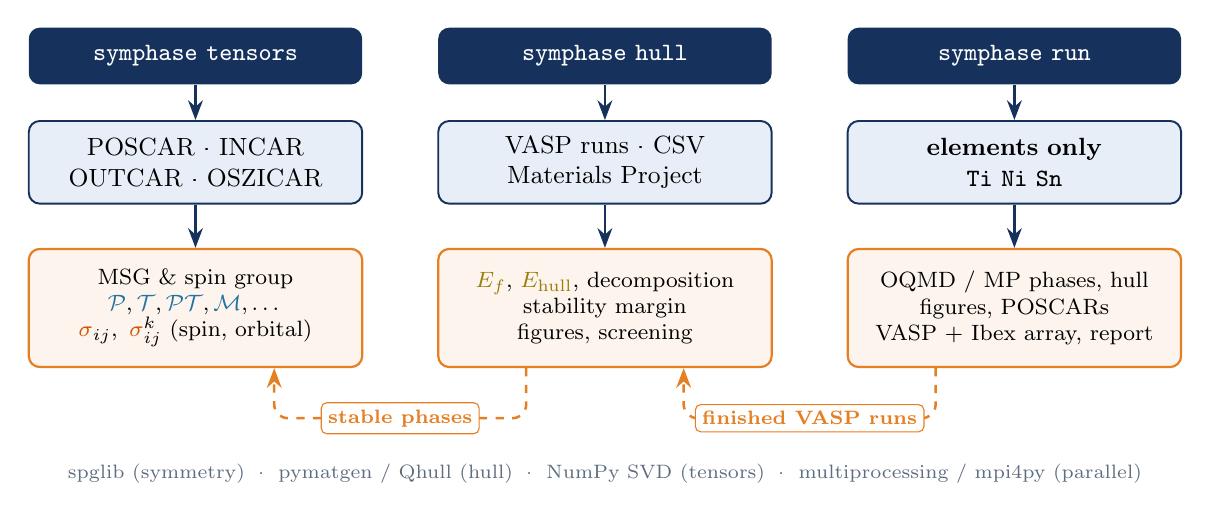
\begin{tikzpicture}[font=\small,
  box/.style={draw=navy,fill=navylight,rounded corners=4pt,text width=4.0cm,minimum height=1.05cm,align=center,line width=0.7pt},
  cmd/.style={fill=navy,text=white,rounded corners=4pt,text width=4.0cm,minimum height=0.72cm,align=center,font=\small\ttfamily\bfseries},
  outb/.style={draw=accent,fill=accent!8,rounded corners=4pt,text width=4.0cm,minimum height=1.5cm,align=center,line width=0.8pt,font=\footnotesize},
  tag/.style={draw=accent,fill=white,rounded corners=2pt,font=\scriptsize\bfseries,text=accent,inner sep=2.5pt},
  arr/.style={-{Stealth[length=2.5mm]},line width=0.9pt,navy},
  fb/.style={-{Stealth[length=2.5mm]},line width=0.9pt,accent,dashed,rounded corners=5pt}]
  \foreach \x/\c/\n in {0/symphase tensors/t, 5.2/symphase hull/h, 10.4/symphase run/r}
    \node[cmd] (\n) at (\x,2.35) {\c};
  \node[box] (ti) at (0,1.0)   {POSCAR · INCAR\\OUTCAR · OSZICAR};
  \node[box] (hi) at (5.2,1.0) {VASP runs · CSV\\Materials Project};
  \node[box] (ri) at (10.4,1.0){\textbf{elements only}\\\texttt{Ti Ni Sn}};
  \node[outb] (to) at (0,-0.85)   {MSG \& spin group\\$\Pop,\Top,\Pop\Top,\Mop,\dots$\\$\sig_{ij},\ \sig^{k}_{ij}$ (spin, orbital)};
  \node[outb] (ho) at (5.2,-0.85) {$\Eform$, $\Ehull$, decomposition\\stability margin\\figures, screening};
  \node[outb] (ro) at (10.4,-0.85){OQMD / MP phases, hull\\figures, POSCARs\\VASP + Ibex array, report};
  \foreach \a/\b in {t/ti,h/hi,r/ri,ti/to,hi/ho,ri/ro} \draw[arr] (\a)--(\b);
  % feedback loops below the output boxes, labels centred on the horizontal legs
  \coordinate (y) at (0,-2.25);
  \coordinate (A1) at ([xshift=-10mm]ro.south); \coordinate (B1) at ([xshift=10mm]ho.south);
  \coordinate (A2) at ([xshift=-10mm]ho.south); \coordinate (B2) at ([xshift=10mm]to.south);
  \draw[fb] (A1) -- (A1 |- y) -- (B1 |- y) -- (B1);
  \draw[fb] (A2) -- (A2 |- y) -- (B2 |- y) -- (B2);
  \node[tag] at ($(A1 |- y)!0.5!(B1 |- y)$) {finished VASP runs};
  \node[tag] at ($(A2 |- y)!0.5!(B2 |- y)$) {stable phases};
  \node[font=\scriptsize,text=greyt] at (5.2,-2.95) {spglib (symmetry) \;·\; pymatgen / Qhull (hull) \;·\; NumPy SVD (tensors) \;·\; multiprocessing / mpi4py (parallel)};
\end{tikzpicture}
\end{frame}

\begin{frame}[fragile]{Installation and quick start}
\begin{columns}[T]
\column{0.57\textwidth}
\textbf{Install}
\begin{lstlisting}[language=bash]
git clone https://github.com/Gokaran-Shukla/symphase
cd symphase && pip install -e .
pip install -e ".[mp,mpi]"   # optional extras
\end{lstlisting}
\textbf{Symmetry and tensors of a VASP run}
\begin{lstlisting}[language=bash]
cd my_vasp_run/ && symphase tensors
symphase tensors --mdir 1 1 0
\end{lstlisting}
\column{0.40\textwidth}
\textbf{Hull from anything}%
\begin{lstlisting}[language=bash]
symphase hull --scan calcs/ -n 40
symphase hull --csv data.csv --bar
\end{lstlisting}
\textbf{Elements in, everything out}
\begin{lstlisting}[language=bash]
symphase run Ti Ni Sn
symphase run symphase.in
\end{lstlisting}
\textbf{Python}
\begin{lstlisting}[language=Python]
from symphase import analyze_tensors
from symphase import HullAnalysis, run
\end{lstlisting}
\end{columns}
\end{frame}

% =============================================================================
\sectionslide{2 \; Magnetic symmetry}{from the VASP files to the magnetic space group}

\begin{frame}{Magnetic space groups in one slide}
\begin{columns}[T]
\column{0.53\textwidth}
Operations $g=\{\Rop|\tau\}$ and $g'=\{\Rop|\tau\}\Top$; moments are \textbf{axial} and $\Top$-odd:
\[
  g:\ \mathbf m \mapsto \det(\Rop)\,\Rop\,\mathbf m,\quad g':\ \mathbf m \mapsto -\det(\Rop)\,\Rop\,\mathbf m
\]
\renewcommand{\arraystretch}{1.25}
\begin{tabular}{@{}lll@{}}
\toprule
type & content & example \\ \midrule
I   & no $\Top$ at all            & colourless \\
II  & $\Top$ itself (grey, $G1'$) & Pt, paramagnets \\
III & $\Top$ with point ops only  & Fe, RuO$_2$ \\
IV  & $\Top\tau$ (antitranslation)& many AFMs \\ \bottomrule
\end{tabular}
\column{0.44\textwidth}
\textbf{Reported by SymPhase}
{\small\begin{itemize}\setlength\itemsep{0.05em}
  \item BNS \& OG symbol/number, UNI number, type
  \item magnetic point group, unitary subgroup
  \item $\Pop$, $\Top$, $\Top\tau$, $\Pop\Top$ present?
  \item mirrors/glides $\Mop$, $\Mop\Top$ (Miller indices)
  \item rotations/screws $C_n$, $C_n\Top$, rotoinversions
  \item every operation + intrinsic translation
\end{itemize}}
\begin{tcolorbox}[hl]
$\Top$ or $\Top\tau$ $\Rightarrow$ all $\Top$-odd responses vanish.
\end{tcolorbox}
\end{columns}
\end{frame}

\begin{frame}{Reading the VASP calculation}
\begin{columns}[T]
\column{0.5\textwidth}
{\small\begin{itemize}\setlength\itemsep{0.2em}
  \item \textbf{POSCAR/CONTCAR}: lattice, species, positions (VASP 4/5)
  \item \textbf{OUTCAR}: ISPIN, LSORBIT, \texttt{SAXIS}, last \texttt{magnetization (x/y/z)} blocks, orbital moments, $E_F$
  \item \textbf{OSZICAR}: ionic steps, $F$, $E_0$, total moment
  \item \textbf{INCAR}: \texttt{MAGMOM}, \texttt{SAXIS}, \texttt{LSORBIT}, \texttt{ISPIN}, \texttt{LDAU}… — POSCAR + INCAR suffice \emph{before} running VASP
  \item non-collinear moments rotated from the \texttt{SAXIS} frame:
  $\mathbf m_{\rm cart} = R_z(\alpha)R_y(\beta)\,\mathbf m_{\rm SAXIS}$
\end{itemize}}
\column{0.46\textwidth}
\textbf{Moment priority}
\begin{enumerate}\setlength\itemsep{0.25em}
  \item \cmd{--magmom} (user, $N$ or $3N$ values)
  \item OUTCAR site moments (last ionic step)
  \item INCAR \texttt{MAGMOM}
  \item MAGMOM echoed in OUTCAR
  \item none $\to$ grey group
\end{enumerate}
\vspace{0.4em}
Collinear runs: $\mathbf m_i = M_i\,\hat{\mathbf n}$, $\hat{\mathbf n}$ = \cmd{--mdir} or \texttt{SAXIS}.\\[0.3em]
Noise control: \cmd{--mmin} (zero small moments), \cmd{--mag-symprec}.
\end{columns}
\end{frame}

% =============================================================================
\sectionslide{3 \; Response tensors}{Neumann's principle, solved numerically}

\begin{frame}{Neumann's principle for magnetic groups}
\[
  \Jc_i = \sig_{ij}\,\Ef_j,\qquad
  \Jc^{\,\Sv_k}_i = \sig^{\,k}_{ij}\,\Ef_j,\qquad
  \Jc^{\,\Lv_k}_i = \sig^{\,k}_{ij}\,\Ef_j
\]
\begin{columns}[T]
\column{0.5\textwidth}
\renewcommand{\arraystretch}{1.3}
\begin{tabular}{@{}lll@{}}
\toprule
tensor & character & $\Dop(\Rop)$\\ \midrule
$\sig_{ij}$ & polar, rank 2 & $\Rop\otimes\Rop$ \\
$\sig^{k}_{ij}$ ($\Sv$) & axial, rank 3 & $\det\Rop\;\Rop\otimes\Rop\otimes\Rop$\\
$\sig^{k}_{ij}$ ($\Lv$) & axial, rank 3 & $\det\Rop\;\Rop\otimes\Rop\otimes\Rop$\\ \bottomrule
\end{tabular}
\vspace{0.4em}

{\small spin current $\{v_i,\Sv_k\}/2$: polar($i$) $\times$ axial($k$), $\Top$-even.}
\column{0.47\textwidth}
\begin{tcolorbox}[sp]
For every $g$ and $g'$ of the magnetic point group:
\[
 \chiT^{\rm even} = \Dop(\Rop)\,\chiT^{\rm even},\qquad
 \chiT^{\rm odd} = \theta_g\,\Dop(\Rop)\,\chiT^{\rm odd}
\]
$\theta_g=+1$ for $g$, $-1$ for $g'$.
\end{tcolorbox}
\textbf{Onsager} (charge only): $\sig_{ij}(\mathbf M)=\sig_{ji}(-\mathbf M)$ $\Rightarrow$
even part symmetric, odd part antisymmetric:
$\sig^{\rm odd}_{ij}=\epsilon_{ijk}h_k$ (Hall vector).
\end{columns}
\end{frame}

\begin{frame}{Algorithm}
\begin{columns}[T]
\column{0.55\textwidth}
\begin{enumerate}\setlength\itemsep{0.55em}
  \item Convert spglib operations to Cartesian: $\Rop_c = A^{T}\Rop A^{-T}$
  \item Stack constraints $\big(\theta_g\Dop(\Rop)-\mathbb 1\big)\,\mathrm{vec}(\chiT)=0$ for all point operations (+ Onsager rows)
  \item Null space by \textbf{SVD} $\to$ basis of allowed tensors
  \item \textbf{Reduced row echelon form} $\to$ independent components (pivots)
  \item Rationalise coefficients ($\tfrac12$, $\sqrt3$, $\tfrac1{\sqrt3}$, …) $\to$ symbolic matrices
\end{enumerate}
\column{0.42\textwidth}
\begin{tcolorbox}[sp,title=Output for each tensor]
\begin{itemize}\setlength\itemsep{0.2em}
  \item 3×3 matrix per spin direction $k$
  \item number of independent components
  \item antisymmetric (SHE-like) vs symmetric (spin-splitter) pairs
  \item conventional ($k\perp i\perp j$) vs \textbf{unconventional} components
  \item allowed $\Sv_k$ for every flow $\perp$ field geometry (SOT)
\end{itemize}
\end{tcolorbox}
\end{columns}
\end{frame}

% =============================================================================
\sectionslide{4 \; Examples}{non-magnetic, ferromagnetic, altermagnetic, low symmetry}

\begin{frame}{fcc Pt (grey group $Fm\bar3m1'$) and bcc Fe ($\mathbf m\parallel z$, $I4/mm'm'$)}
\begin{columns}[T]
\column{0.47\textwidth}
\textbf{Pt} — $\Top$ present: every $\Top$-odd tensor vanishes.\\[0.3em]
Spin Hall ($\Top$-even), \textbf{one} component:
\[
\sig^{\,z}=\begin{pmatrix}0&\sig^{x}_{yz}&0\\-\sig^{x}_{yz}&0&0\\0&0&0\end{pmatrix},\quad
\sig^{\,k}_{ij}=\sig_{\rm SH}\,\epsilon_{kij}
\]
\column{0.5\textwidth}
\textbf{Fe} — MPG $4/mm'm'$, $\Pop$ yes, $\Top$ no.
\[
\sig^{\rm odd}=\begin{pmatrix}0&\sig_{xy}&0\\-\sig_{xy}&0&0\\0&0&0\end{pmatrix}
\ \Rightarrow\ \mathbf h\parallel\hat z\ \ \text{(AHE)}
\]
Magnetic SHE: 4 independent $\Top$-odd components,
e.g.\ $\sig^{\,z}_{xx},\ \sig^{\,z}_{zz},\ \sig^{\,x}_{xz}$ — spin $\parallel\mathbf m$.
\end{columns}
\vfill
\begin{tcolorbox}[hl]
Same code path for both: only the moments differ. Moments come straight from the OUTCAR (non-collinear, SAXIS-rotated).
\end{tcolorbox}
\end{frame}

\begin{frame}{Altermagnetic RuO$_2$: the Néel vector decides}
\begin{columns}[T]
\column{0.58\textwidth}
\renewcommand{\arraystretch}{1.3}\small\setlength{\tabcolsep}{4pt}
\begin{tabular}{@{}lllcl@{}}
\toprule
Néel & MSG (BNS) & MPG & AHE & Hall vector $\mathbf h$ \\ \midrule
$[001]$ & $P4_2'/mnm'$ & $4'/mmm'$ & -- & 0 \\
$[100]$ & $Pnn'm'$ & $mm'm'$ & \textcolor{spinc}{\checkmark} & $(0,-\sig_{xz},0)$ \\
$[110]$ & $Cmm'm'$ & $mm'm'$ & \textcolor{spinc}{\checkmark} & $(-\sig_{xz},-\sig_{xz},0)$ \\ \bottomrule
\end{tabular}
\vspace{0.6em}

\textbf{Spin splitter} (Néel $\parallel[001]$, $\Top$-odd):
\[
\sig^{\,z}_{\rm odd}=\begin{pmatrix}0&\sig^{z}_{xy}&0\\ \sig^{z}_{xy}&0&0\\0&0&0\end{pmatrix}
\]
symmetric $\Rightarrow$ not a spin Hall effect.
\column{0.36\textwidth}
\begin{tcolorbox}[sp]
\texttt{symphase tensors} \\ \texttt{\;\;--mdir 1 1 0}\\[0.3em]
rotates collinear moments: one VASP run, all orientations.
\end{tcolorbox}
\begin{tcolorbox}[hl]
SymPhase flags \emph{compensated, no $\Pop\Top$, no $\Top\tau$} $\Rightarrow$ altermagnet-like.
\end{tcolorbox}
\end{columns}
\end{frame}

\begin{frame}{Low symmetry: monoclinic MoO$_2$ ($P2_1/c$, MPG $2/m1'$)}
\begin{columns}[T]
\column{0.40\textwidth}
{\small Non-magnetic distorted rutile, unique axis $b\parallel y$; POSCAR + INCAR only.}\\[0.5em]
\textbf{Charge} (4 independent):
\[
\sig=\begin{pmatrix}\sig_{xx}&0&\sig_{xz}\\0&\sig_{yy}&0\\\sig_{xz}&0&\sig_{zz}\end{pmatrix}
\]
\begin{tcolorbox}[sp]
$\textcolor{opc}{C_{2y}}:\ x\to-x,\ z\to-z$ (axial tensor)\\[0.2em]
$\sig^{k}_{ij}\neq0 \iff$ \textbf{odd number of $y$}\\
$\Rightarrow$ \textbf{13} independent $\sig^{k}_{ij}$ for $\Sv$ and $\Lv$
\end{tcolorbox}
\column{0.57\textwidth}
\textbf{Spin Hall tensor} ($\Top$-even), $\Jc^{\,\Sv_k}_i=\sig^{k}_{ij}\Ef_j$:
{\footnotesize
\[
\sig^{\,x}=\begin{pmatrix}0&\sig^{x}_{xy}&0\\ \sig^{x}_{yx}&0&\sig^{x}_{yz}\\0&\sig^{x}_{zy}&0\end{pmatrix}\!,\quad
\sig^{\,y}=\begin{pmatrix}\sig^{y}_{xx}&0&\sig^{y}_{xz}\\0&\sig^{y}_{yy}&0\\ \sig^{y}_{zx}&0&\sig^{y}_{zz}\end{pmatrix}
\]
\vspace{-0.4em}
\[
\sig^{\,z}=\begin{pmatrix}0&\sig^{z}_{xy}&0\\ \sig^{z}_{yx}&0&\sig^{z}_{yz}\\0&\sig^{z}_{zy}&0\end{pmatrix}
\]}
\vspace{-0.6em}
\begin{columns}[T]
\column{0.48\linewidth}
{\small\renewcommand{\arraystretch}{1.05}
\begin{tabular}{@{}lll@{}}
\toprule
flow & field & allowed $\Sv$ \\ \midrule
$x$ & $\Ef\parallel y$ & $\Sv_z$, \textcolor{accent}{$\Sv_x$} \\
$z$ & $\Ef\parallel y$ & $\Sv_x$, \textcolor{accent}{$\Sv_z$} \\
$z$ & $\Ef\parallel x$ & $\Sv_y$ \\ \bottomrule
\end{tabular}\\[0.1em]
{\scriptsize\textcolor{accent}{orange} = unconventional}}
\column{0.5\linewidth}
\begin{tcolorbox}[hl,halign=flush left]
\textbf{No SOC:} all $\sig^{k}_{ij}(\Sv)\to0$;\\ the 13 $\sig^{k}_{ij}(\Lv)$ survive.
\end{tcolorbox}
\end{columns}
\end{columns}
\end{frame}

\begin{frame}{Spin groups: symmetry without spin–orbit coupling}
\begin{columns}[T]
\column{0.53\textwidth}
Without SOC spin and lattice rotate \textbf{independently}: elements $[\textcolor{spinc}{U}\,\|\,g]$,
$\textcolor{spinc}{U}\in O(3)$, $g=\{\Rop|\tau\}$ (improper $\textcolor{spinc}{U}$ = rotation $\times\,\Top$):
\[
 g\in\text{spin group}\iff \exists\,\textcolor{spinc}{U}:\ \mathbf m_{g(i)}=\textcolor{spinc}{U}\,\mathbf m_i\ \ \forall i
\]
\textcolor{spinc}{U} by orthogonal Procrustes (SVD), plus the \textbf{spin-only group}: $O(3)$, $^{\infty}m1$ (collinear), $^{m}1$ (coplanar).\\[0.4em]
Tensors with $\textcolor{spinc}{U}=\theta\,\textcolor{spinc}{Q}$, $\theta=\det \textcolor{spinc}{U}$:
\[
\sig^{k}_{ij}:\ \Dop=\textcolor{spinc}{Q}\otimes\Rop\otimes\Rop,\quad
\sig^{k}_{ij}(\Lv):\ \Dop=\det\Rop\,\Rop\otimes\Rop\otimes\Rop
\]
\column{0.44\textwidth}
\begin{tcolorbox}[sp,title=Reported (\texttt{--analysis spin})]
\begin{itemize}\setlength\itemsep{0.15em}
 \item operations $[\textcolor{spinc}{U}\|g]$, cosets $H$ / $A$
 \item magnet class: FM, AFM ($[C_2\|\tau]$), PT-AFM ($[C_2\|\Pop]$), \textbf{altermagnet}
 \item spin Laue group, e.g.\ $^{2}4/^{1}m\,^{2}m\,^{1}m$
 \item spin splitting $\textcolor{spinc}{\mathbf s}(\mathbf k)$ from $\textcolor{spinc}{\mathbf s}(\theta\Rop\mathbf k)=\theta \textcolor{spinc}{Q}\,\textcolor{spinc}{\mathbf s}(\mathbf k)$: d/g/i-wave, nodal planes
 \item NR tensors and \textbf{SOC-only} components
\end{itemize}
\end{tcolorbox}
\end{columns}
\end{frame}

\begin{frame}{Spin-group classification of the examples}
\renewcommand{\arraystretch}{1.25}\centering\small
\begin{tabular}{@{}llllp{3.9cm}@{}}
\toprule
system & magnet class & spin Laue group & NR splitting & $\textcolor{spinc}{\mathbf s}(\mathbf k)$ / remark \\ \midrule
RuO$_2$ (Néel $\parallel z$) & \textbf{altermagnet} & $^{2}4/^{1}m\,^{2}m\,^{1}m$ & d-wave & $s_z\propto k_xk_y$, 2 nodal planes \\
MnTe (NiAs) & \textbf{altermagnet} & $^{2}6/^{2}m\,^{1}m\,^{2}m$ & g-wave & $s_z\propto k_z k_y(k_y^2-3k_x^2)$ \\
bcc Cr & AFM, $[C_2\|\tau]$ & — & none & Kramers degenerate \\
Mn$_2$Au & PT-AFM, $[C_2\|\Pop]$ & — & none & Kramers degenerate \\
bcc Fe & ferromagnet & $^{1}4/^{1}m\,^{1}\bar3\,^{1}m$ & s-wave & Zeeman-like \\
fcc Pt & non-magnetic & — & none & spin decoupled \\ \bottomrule
\end{tabular}
\vspace{0.6em}
\begin{tcolorbox}[hl]
RuO$_2$ without SOC: spin splitter $\sig^{z}_{xy}=+\sig^{z}_{yx}$ ($\Top$-odd) survives; the spin Hall effect is \textbf{SOC-only};
the orbital Hall effect needs no SOC. Moments for MnTe, Cr, Mn$_2$Au come from the INCAR alone.
\end{tcolorbox}
\end{frame}

\begin{frame}{Spin-space-group numbers}
\begin{columns}[T]
\column{0.44\textwidth}
Collinear SSG $=\{[E\|h]\}\cup\{[\textcolor{spinc}{C_{2\perp}}\|a]\}\;\otimes\;^{\infty}m1$.\\[0.3em]
Replacing $\textcolor{spinc}{C_{2\perp}}\to\Top$ maps it one-to-one onto a black-and-white group of type I, III or IV:
\[
230+674+517=\mathbf{1421}\ \text{collinear SSGs}
\]
\begin{tcolorbox}[sp]
SymPhase: spglib on the scalar moments $\mathbf m_i\!\cdot\hat{\mathbf n}$ $\to$ BNS number;
cross-checked with \texttt{spinspg}. Non-collinear: lattice group, spin-preserving subgroup, spin point group.
\end{tcolorbox}
\column{0.53\textwidth}
\renewcommand{\arraystretch}{1.2}\small
\begin{tabular}{@{}lll@{}}
\toprule
system & collinear SSG (BNS) & spin Laue \\ \midrule
RuO$_2$ & $P4_2'/mn'm$ \;136.498 & $^{2}4/^{1}m\,^{2}m\,^{1}m$ \\
MnTe & $P6_3'/m'mc'$ \;194.269 & $^{2}6/^{2}m\,^{1}m\,^{2}m$ \\
bcc Cr & $P_Im\bar3m$ \;221.97 (IV) & — \\
Mn$_2$Au & $I4/m'mm$ \;139.533 & — \\
bcc Fe & $Im\bar3m$ \;229.140 (I) & $^{1}4/^{1}m\,^{1}\bar3\,^{1}m$ \\ \bottomrule
\end{tabular}
\vspace{0.5em}

{\small Primes in the SSG symbol = $^{2}$ in the spin Laue group: two independent routes agree.}
\end{columns}
\end{frame}

\begin{frame}{Magnon chirality splitting (linear spin-wave theory)}
\noindent{\footnotesize $H=\sum J_{ij}\,\Sv_i\!\cdot\!\Sv_j-K\sum(\Sv_i\!\cdot\!\hat{\mathbf n})^2$; bonds grouped by \textbf{crystal symmetry}
(RuO$_2$: 6.35 Å bonds along [110] and [1$\bar1$0] inequivalent); Colpa diagonalisation, each mode $\Delta\Sv_z=\pm1$ ($\alpha$/$\beta$).}
\vspace{0.3em}

\centering
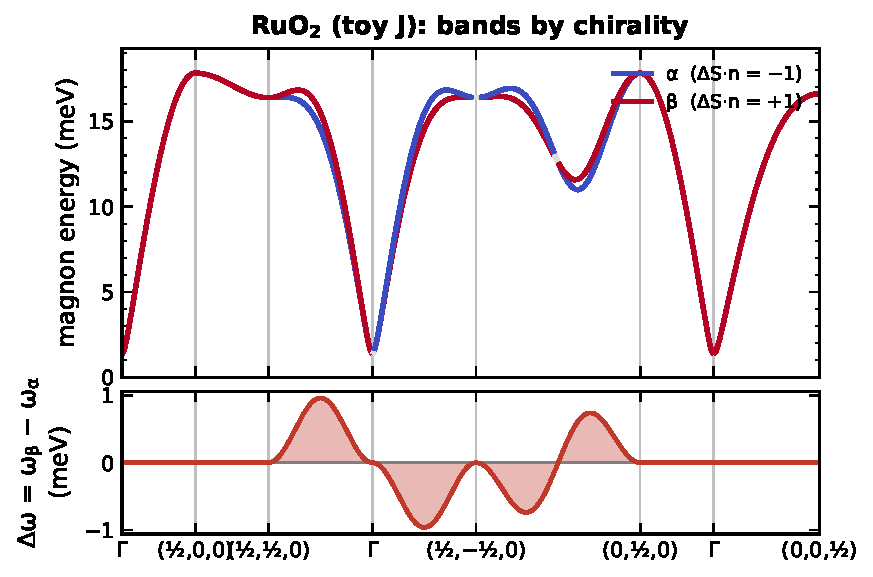
\includegraphics[height=0.47\textheight]{figures/magnon_bands.pdf}\hspace{0.6em}
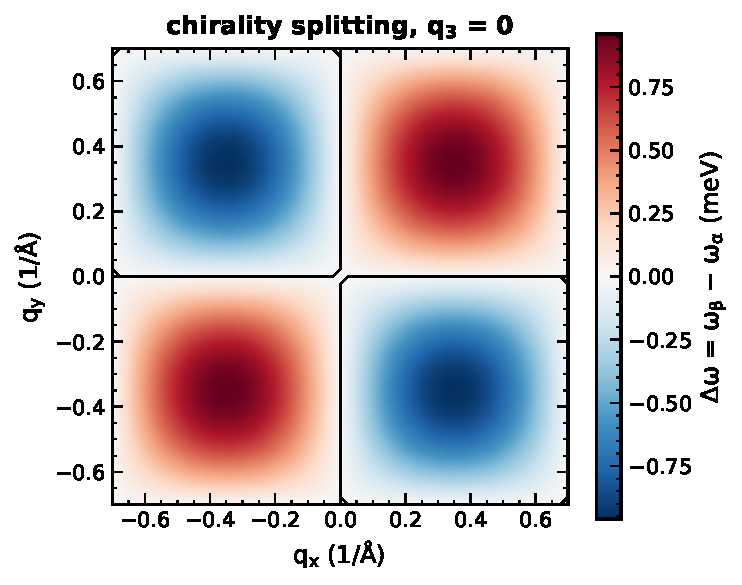
\includegraphics[height=0.47\textheight]{figures/magnon_map.pdf}

\vspace{0.2em}
\begin{tcolorbox}[hl,width=0.94\textwidth]
$\Delta\omega=\omega_\beta-\omega_\alpha\propto q_xq_y$: \textbf{d-wave}, the same form as the spin-group $\textcolor{spinc}{s_z}(\mathbf k)\propto k_xk_y$.
Tests: FM and AFM chain exact; $J_7=J_8\Rightarrow\Delta\omega=0$. {\scriptsize (toy $J$; \texttt{symphase magnons --J ...} or \texttt{--exchange J.dat})}
\end{tcolorbox}
\end{frame}

\begin{frame}{Non-collinear ferro- and antiferromagnets}
\begin{columns}[T]
\column{0.42\textwidth}
{\footnotesize
\textbf{Symmetry:} $U$ in $[U\|g]$ by Procrustes fit; spin-only group $\{E,C_2(\hat{\mathbf n})\Top\}$ (coplanar) or trivial.
Classes: non-collinear AFM (compensated) or ferro/ferrimagnet (canted, weak FM).\\[0.4em]
\textbf{LSWT in local frames} (Toth \& Lake 2015), $H=\sum\Sv_i^{T}J_{ij}\Sv_j+\sum\Sv_i^{T}A_i\Sv_i$ with Heisenberg, DMI or full tensors:
\[
A_{ij}\ni\tfrac{\sqrt{S_iS_j}}{2}\,\mathbf u_i^{T}J_{ij}\bar{\mathbf u}_j e^{i\mathbf k\cdot\mathbf d},\
B_{ij}\ni\tfrac{\sqrt{S_iS_j}}{2}\,\mathbf u_i^{T}J_{ij}\mathbf u_j e^{i\mathbf k\cdot\mathbf d}
\]
magnon spin vector $\Delta\mathbf S_n$ per mode, non-reciprocity, \texttt{--relax} to the classical ground state.}
\column{0.56\textwidth}
\centering{\small\textbf{120° triangular AFM}}\\
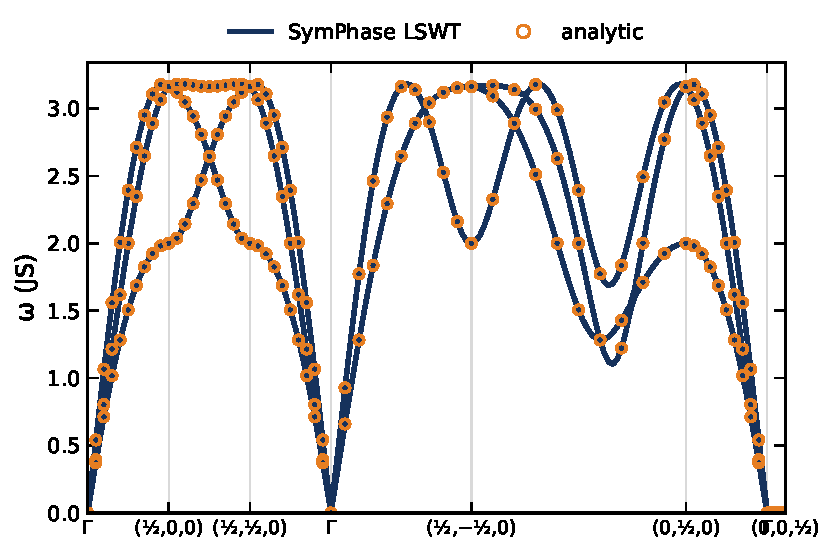
\includegraphics[width=0.84\linewidth]{figures/triangular.pdf}
{\scriptsize\renewcommand{\arraystretch}{1.05}
\begin{tabular}{@{}p{0.36\linewidth}p{0.60\linewidth}@{}}
\toprule
test & result \\ \midrule
FM $\parallel[111]$ vs $\parallel z$ & identical spectra ($10^{-15}$ meV) \\
120° triangular AFM & analytic to $10^{-4}$; 3 Goldstone modes \\
DMI chain & $\arctan(D/J)=11.31^\circ$ canting, weak FM \\ \bottomrule
\end{tabular}}
\end{columns}
\end{frame}

\begin{frame}{Incommensurate spirals without supercells}
\noindent{\footnotesize Single-Q planar spiral $\Sv_j(\mathbf R)=R_{\hat{\mathbf n}}(\mathbf q\cdot\mathbf R)\,\Sv_j(\mathbf 0)$. If $H$ is invariant under
rotations about $\hat{\mathbf n}$ (Heisenberg, $\mathbf D\parallel\hat{\mathbf n}$, anisotropy along $\hat{\mathbf n}$), the order is periodic in the
\textbf{rotating frame}:\quad $J_{ij}(\mathbf R)\to J_{ij}(\mathbf R)\,R_{\hat{\mathbf n}}(2\pi\,\mathbf q\cdot\mathbf R)$, and LSWT runs on the original cell.
$\mathbf q$ from minimising the classical $E(\mathbf q,\psi_i)$; \texttt{--relax} warns when a spiral beats the fixed cell.}
\vspace{0.3em}

\centering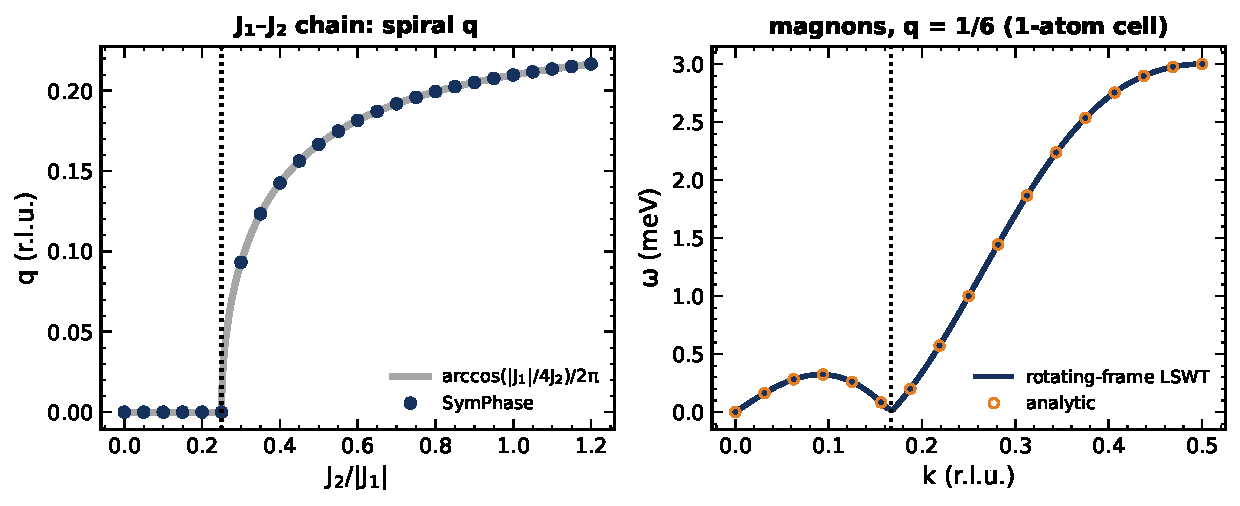
\includegraphics[width=0.70\textwidth]{figures/spiral.pdf}

{\scriptsize\renewcommand{\arraystretch}{1.0}
\begin{tabular}{@{}p{0.2\textwidth}p{0.48\textwidth}p{0.24\textwidth}@{}}
\toprule
J$_1$–J$_2$ chain & $q=1/6$, $E=-0.75$ meV; $\omega(k)$ = analytic ($4\times10^{-5}$) & = 6-site supercell \\
DMI helix, $D/|J|=0.2$ & $q=\arctan(D/|J|)/2\pi=0.0314$: period 95.5 Å $=31.8\,a$ & sense set by sign of $D$ \\ \bottomrule
\end{tabular}}
\end{frame}

\begin{frame}{Beyond the rotating frame: magnetic supercells}
\begin{columns}[T]
\column{0.53\textwidth}
\footnotesize
\textbf{Needs a supercell:} multi-Q (skyrmion crystals), conical spirals (field $\parallel\hat{\mathbf n}$),
spirals distorted by in-plane anisotropy (3$q$, 5$q$), non-invariant $J$ tensors.
\texttt{--spiral} refuses these and points to \texttt{--supercell auto}:
\begin{enumerate}\setlength\itemsep{0.12em}
  \item \textbf{Luttinger–Tisza}: $\min_{\mathbf q}\lambda_{\min}[J(\mathbf q)]$ $\to$ $\mathbf q_{LT}$ + star
  \item \textbf{size}: smallest $n_1\!\times\! n_2\!\times\! n_3$ fitting every star member ($n\times n$ for hexagonal)
  \item exact \textbf{mapping} of $J$, $A$, $\mathbf B$ (Zeeman $-g\mu_B\mathbf B\cdot\Sv$)
  \item \textbf{L-BFGS} from many seeds: LT single-Q, conical, multi-Q, random
  \item \textbf{identify}: structure factor, harmonics, $w(0)$, $N_{sk}$
  \item \textbf{LSWT} in the supercell (stability, folded bands)
  \item \texttt{POSCAR}/\texttt{INCAR}/\texttt{J\_super.dat} $\to$ VASP \& \texttt{symphase tensors}
\end{enumerate}
\column{0.43\textwidth}
\begin{tcolorbox}[sp,title=Commands]
\raggedright\scriptsize\ttfamily
symphase magnons ... --supercell auto\\
\quad --field 0 0 14\\
\quad --K 0.4 --K-axis 1 0 0\\
\quad --scan 4 15 {\rmfamily (size convergence)}\\
\quad --supercell 7 1 1 {\rmfamily (fixed size)}
\end{tcolorbox}
\begin{tcolorbox}[hl,title=Size scan: incommensurate $q$]
\raggedright\scriptsize $J_2=0.4$, $q=0.14255$: $E(n)$ lowest at $n=7$ (and 14),
$-0.712498$ vs.\ exact $-0.712500$ meV.\\[0.2em]
Guide: \texttt{docs/SUPERCELL\_WORKFLOW.md}
\end{tcolorbox}
\end{columns}
\end{frame}

\begin{frame}{Supercell results: skyrmion crystal, cone, distorted spiral}
\centering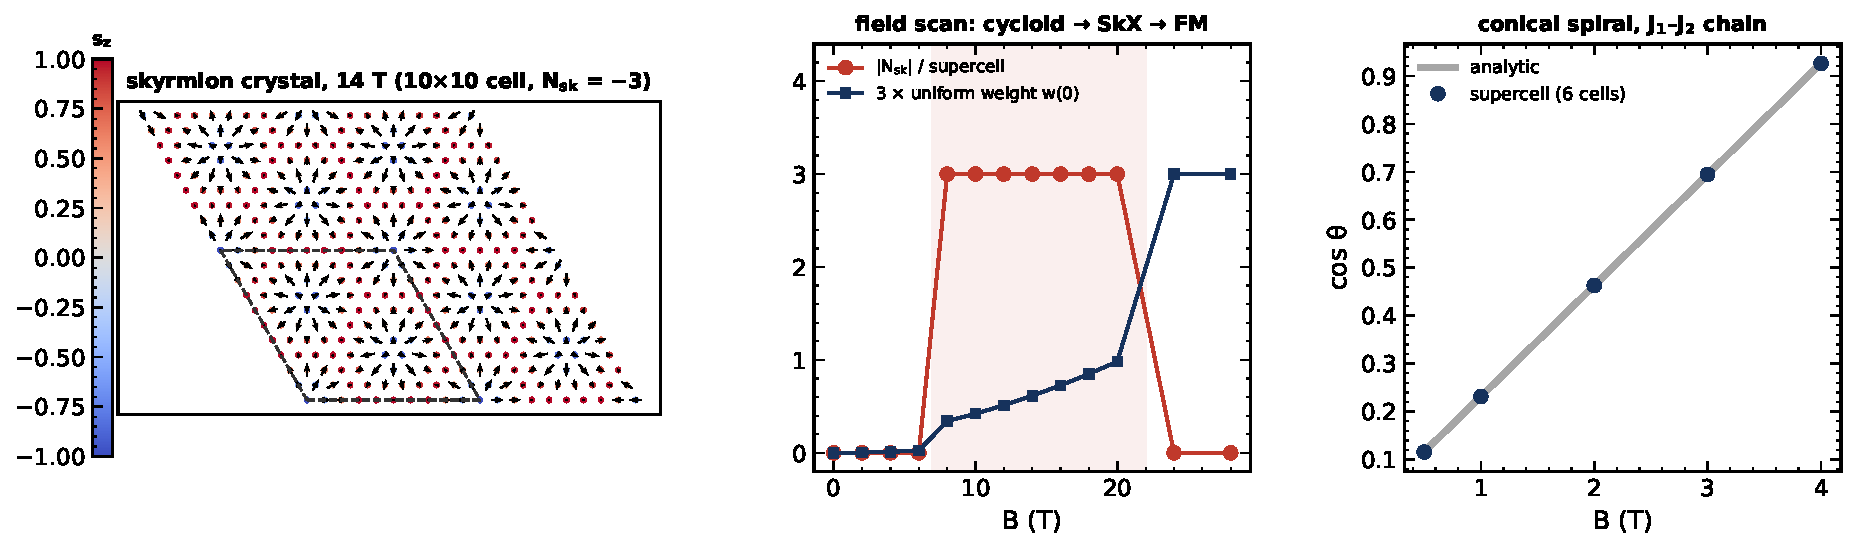
\includegraphics[width=0.98\textwidth]{figures/supercell.pdf}

{\scriptsize\renewcommand{\arraystretch}{1.0}
\begin{tabular}{@{}>{\raggedright\arraybackslash}p{0.27\textwidth}>{\raggedright\arraybackslash}p{0.52\textwidth}>{\raggedright\arraybackslash}p{0.17\textwidth}@{}}
\toprule
triangular FM + DMI, field & 10$\times$10 cell, 3$Q$ + $w(0)$, $N_{sk}=-3$ (8–20 T); $P6m'm'$ & $\sigma_{xy}$ allowed \\
J$_1$–J$_2$ chain, $B=2$ T & cone: $\cos\theta=0.46307$ = analytic & 1 Goldstone mode \\
J$_1$–J$_2$ + easy axis $K=0.4$ & distorted spiral, 3$q$ weight 0.015, locked at 6$a$ & below planar spiral \\ \bottomrule
\end{tabular}}
\end{frame}

\begin{frame}{Spin-space-group numbers for every magnetic order}
\noindent{\footnotesize Collinear SSGs: SymPhase's own label (BNS number of the $C_{2\perp}\!\to\!\Top$ group, 1421 groups).
\textbf{Any} order — collinear, coplanar, non-coplanar — now also gets the \textbf{oriented SSG number} of Chen \emph{et al.},
PRX \textbf{14}, 031038 (2024), via their FindSpinGroup package; its SOC magnetic group is checked against SymPhase's spglib result.}
\vspace{0.4em}

\centering{\scriptsize\renewcommand{\arraystretch}{1.1}\setlength{\tabcolsep}{4pt}
\begin{tabular}{@{}llllll@{}}
\toprule
example & order & OSSG index & spin PG & MSG (FSG) & SymPhase\\ \midrule
RuO$_2$ & collinear altermagnet & \texttt{136.65.1.1.L} & $\infty/mm$ & 136.499 & 136.499 \textcolor{spinc}{\checkmark}\\
MnTe & collinear altermagnet & \texttt{194.164.1.1.L} & $\infty/mm$ & 194.268 & 194.268 \textcolor{spinc}{\checkmark}\\
Mn$_3$Sn & coplanar 120° & \texttt{194.6.1.1.P} & $6/mmm$ & 194.271 & 194.271 \textcolor{spinc}{\checkmark}\\
triangular 120° AFM & coplanar & \texttt{191.187.3.1.P} & $\bar62m$ & 189.223 & 189.223 \textcolor{spinc}{\checkmark}\\
canted DMI chain & coplanar FM & \texttt{123.123.2.2.P2} & $mm2$ & 51.295 & 51.295 \textcolor{spinc}{\checkmark}\\
skyrmion crystal & non-coplanar & \texttt{191.6.1.2} & $6mm$ & 183.189 & 183.189 \textcolor{spinc}{\checkmark}\\ \bottomrule
\end{tabular}}
\vspace{0.5em}

\begin{tcolorbox}[sp,width=0.92\textwidth]
\footnotesize $L_0$ of the index = SymPhase's spin-preserving subgroup $H$ (RuO$_2$: Cmmm, MnTe: $P\bar3m1$).
\quad \cmd{symphase tensors} prints it automatically (\cmd{--ossg auto|yes|no}; \texttt{pip install findspingroup}).
\end{tcolorbox}
\end{frame}

\begin{frame}{Magnon–phonon coupling and quasi-harmonic / anharmonic hulls}
\begin{columns}[T]
\column{0.5\textwidth}
\footnotesize
\textbf{Magnon polarons.} Spins $(X,Y)$ + lattice $(u,P)$ as one harmonic system;
$J(\mathbf d)=J+\sum_\gamma G^\gamma\delta d_\gamma$ $\Rightarrow$
$\partial^2E/\partial X_a\partial u_{j\gamma}=\sqrt{S_a}S_b\,\mathbf x_a\!\cdot\! G^\gamma\!\cdot\mathbf v_b$;
symplectic diagonalisation. Isotropic striction couples only non-collinear spins.
\column{0.46\textwidth}
\footnotesize
\textbf{QHA + anharmonic.} $G(T)=\min_V[E(V)+F_\text{vib}(V,T)+F_\text{anh}]$;
phonopy tables or Debye–Grüneisen $\theta(V)$; $F_\text{anh}=-\tfrac32k_BaT^2$; \cmd{--vib qha|qha-debye}.
\end{columns}
\vspace{0.2em}

\centering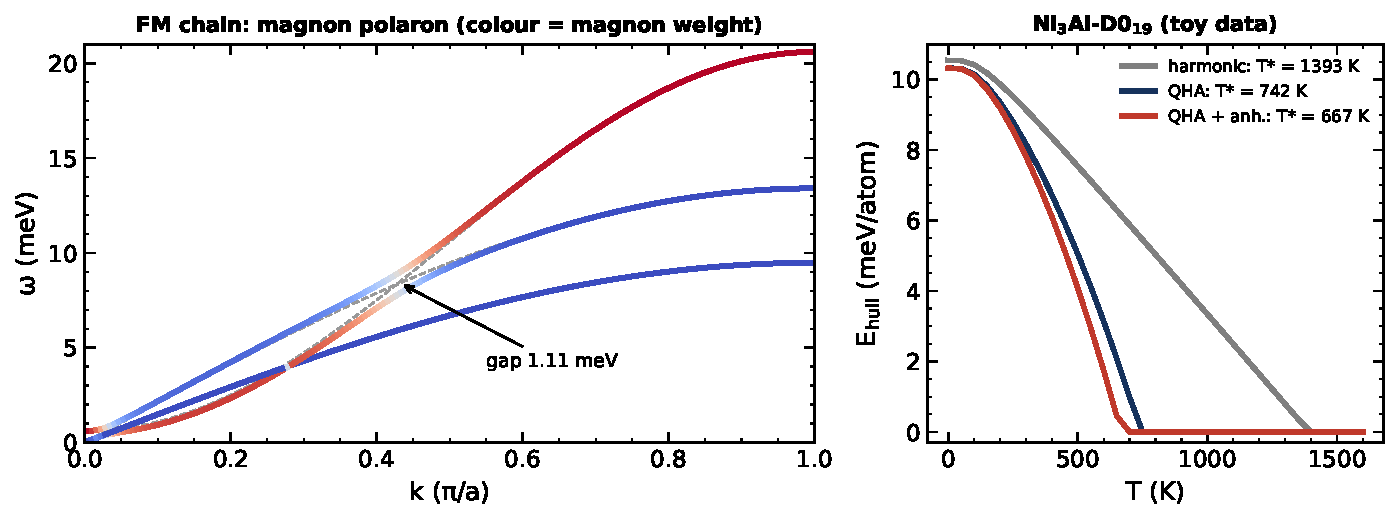
\includegraphics[width=0.74\textwidth]{figures/magphon_qha.pdf}

{\tiny Checks: two-oscillator formula ($3\times10^{-14}$ meV), phonopy $\Phi(\mathbf k)$ = springs ($10^{-12}$), \texttt{PhonopyQHA}: $V$ to $2\times10^{-4}$ Å$^3$, $G$ to $10^{-6}$ eV.}
\end{frame}

\begin{frame}{Magnitudes: Wannier-based Kubo codes, constrained by symmetry}
\begin{columns}[T]
\column{0.52\textwidth}
\footnotesize
Symmetry gives the shape of $\sig$; Kubo gives the size. \cmd{symphase kubo}:
\begin{itemize}\setlength\itemsep{0.15em}
  \item \textbf{plan}: pivot components + postw90 blocks (\texttt{shc\_alpha/beta/gamma}) + a check component
  \item \textbf{import}: postw90 AHC/SHC Fermi scans, any \texttt{component value} table (OHC codes)
  \item \textbf{fit}: independent parameters $\to$ full tensor; violation and forbidden non-zero components flagged
  \item \textbf{compute}: built-in Kubo on \texttt{hr.dat} (AHC, SHC) for the pivots only
\end{itemize}
$\sig_{ij}=-\tfrac{e^2}{\hbar}\!\int\!\sum_nf_n\Omega_{n,ij}$, \ spin: $\partial_iH\to\tfrac12\{\sigma_k,\partial_iH\}$.
\column{0.44\textwidth}
\begin{tcolorbox}[sp,title=Checks]
\scriptsize
Haldane $|\sig_{xy}|=1\,e^2/h$; trivial phase 0\\
Kane–Mele $|\sig^z_{xy}|=1\,(\hbar/e)e^2/h$, $\sig_{xy}=0$\\
3D stack: 774.809 S/cm $=(e^2/h)/c$\\
check component: $10^{-13}$ relative\\
Pt: one postw90 number $\to$ 6 components\\
Fe: forbidden $\sig_{yz},\sig_{zx}$ flagged (0.27\,\%)
\end{tcolorbox}
\end{columns}
\end{frame}

\begin{frame}{Self-consistent anharmonic phonons: TDEP and SSCHA input}
\noindent{\footnotesize $F(T)=F_\text{ph}[\omega_\text{eff}(T)]+\langle V-V_\text{eff}\rangle$. Readers: TDEP folders (\texttt{outfile.free\_energy} +
2nd value of \texttt{outfile.U0}), SSCHA / any $T$–$F$ table (eV, meV, Ry, Ha, kJ/mol; per atom or cell). Smooth $F(T)$, $S=-\partial F/\partial T$;
anharmonic QHA over volumes; hull \cmd{--vib scph} (\texttt{e\_static} when $F$ contains the static energy).}
\vspace{0.3em}

\centering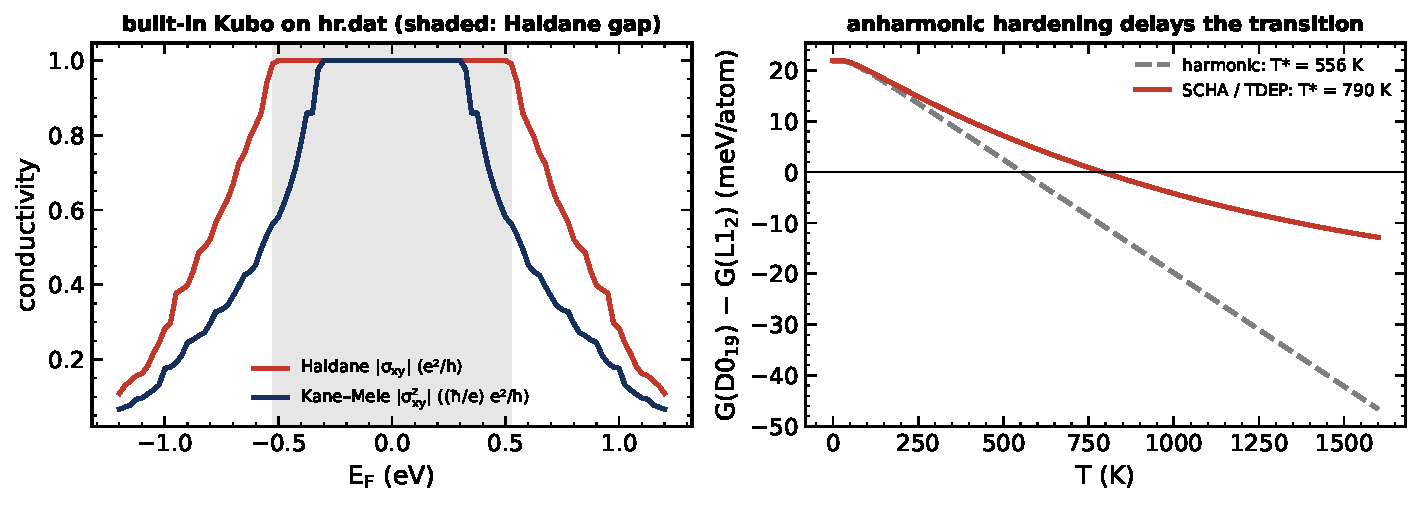
\includegraphics[width=0.78\textwidth]{figures/kubo_scph.pdf}

{\tiny Quartic oscillator at 1000 K: SCHA $-$ exact $=+0.22$ meV ($\ge0$, Gibbs–Bogoliubov), harmonic $-5.07$ meV. Toy Ni$_3$Al-D0$_{19}$: $T^*$ 556 K (harmonic) $\to$ 790 K (SCHA).}
\end{frame}

\begin{frame}{Two-magnon striction and damping of magnons and phonons}
\noindent{\footnotesize $\partial J/\partial d$ in the \emph{bilinear} magnon Hamiltonian: $H_3=N^{-1/2}\sum(b_{\mathbf q}+b^\dagger_{-\mathbf q})\,\Psi^\dagger_{\mathbf k+\mathbf q}M(\mathbf k,\mathbf q)\Psi_{\mathbf k}$
— magnon scattering, phonon $\to$ two magnons; also for collinear spins. Golden-rule linewidths at $T$; Gilbert $\alpha$ + lattice friction $\eta$ via
exact linearised LLG. \cmd{--linewidth T --alpha --phonon-damping}.}
\vspace{0.25em}

\centering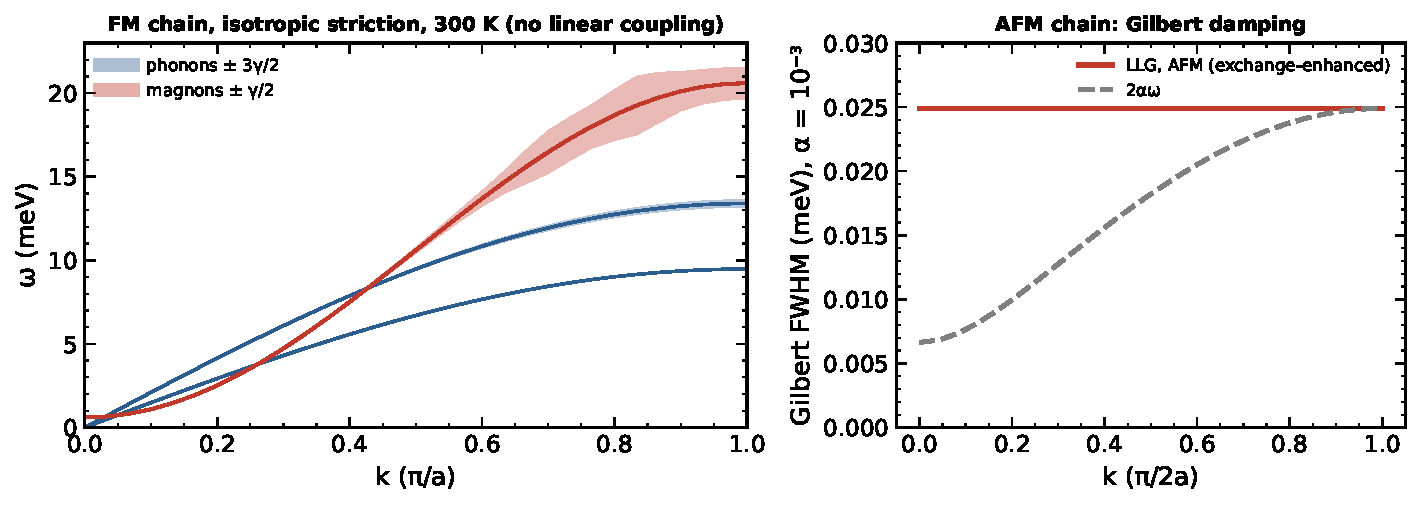
\includegraphics[width=0.80\textwidth]{figures/damping.pdf}

{\tiny Vertex = frozen-phonon supercell to $10^{-11}$ (all blocks); 1D BZ sum = semi-analytic root formula ($10^{-5}$); FM: $\gamma=2\alpha\omega/(1+\alpha^2)$ exactly;
AFM: LLG = energy-dissipation formula, $\gamma=2\alpha(2J+2K)S$; AFM optical phonon decays into two magnons at $T=0$.}
\end{frame}

\begin{frame}{Magnon--magnon interactions and self-energies beyond the golden rule}
\noindent{\footnotesize Holstein--Primakoff to quartic order in local frames, Wick (Hartree--Fock) decoupling with thermal $\langle a^\dagger a\rangle,\langle aa\rangle$:
first order $=\textcolor{spinc}{1/S}$ correction, or self-consistent. From the vertex $M(\mathbf k,\mathbf q)$: complex $\textcolor{red!70!black}{\Sigma(\omega)}$ and
$A(\omega)=-\frac1\pi\mathrm{Im}\,[\omega-\omega_0-\textcolor{red!70!black}{\Sigma(\omega)}]^{-1}$. \cmd{--hf T [--hf-order sc]}, \cmd{--spectral}.}
\vspace{0.25em}

\centering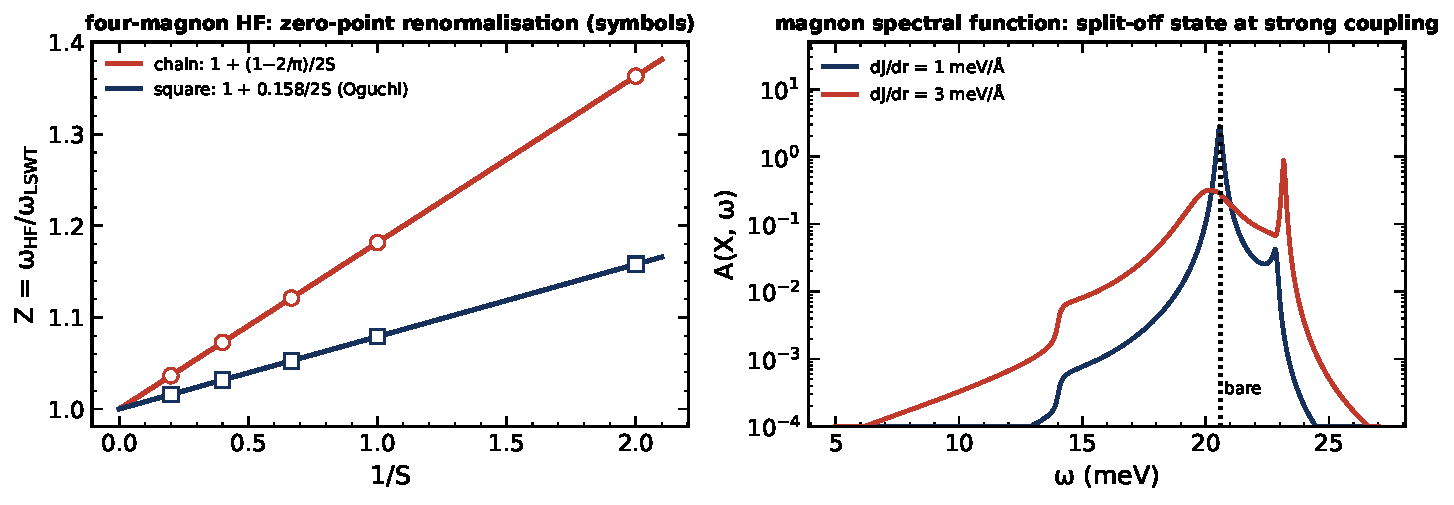
\includegraphics[width=0.84\textwidth]{figures/interactions.pdf}

{\tiny Dyson FM ($T$-softening) exact; Oguchi $Z=1+(1-2/\pi)/2S$ (chain), $Z_c=1.15795$ (square, $S=\frac12$); 1D $\langle S^z\rangle$ diverges, SC-HF breaks down (Mermin--Wagner);
$-2\,\mathrm{Im}\,\Sigma(\omega_0)=\gamma_{\rm golden}$ to $10^{-12}$, $\int A=1$; strong coupling: split-off state above the emission continuum (weight 0.22).}
\end{frame}

\begin{frame}{Cubic magnon terms and second-order four-magnon damping}
\noindent{\footnotesize Non-collinear: $(S-n_i)\,\mathbf v_i\!\cdot\!J\!\cdot\!\mathbf S_j^\perp\to$ \textcolor{red!70!black}{$H_3$}; one-loop bubble + tadpole $=$ the rest of the
\textcolor{spinc}{$1/S$} spectrum, spontaneous decay $\Gamma^{(3)}$ at $T=0$. Quartic vertex at 2nd order (sunset): thermal $2\!\leftrightarrow\!2$ damping $\Gamma^{(4)}$.
$\Sigma(\omega)=r!\sum|c|^2[\prod_{\rm cr}(1{+}n)\prod_{\rm an}n-\prod_{\rm cr}n\prod_{\rm an}(1{+}n)]/(\omega-E+i\eta)$. \cmd{--hf T --cubic --damping4}.}
\vspace{0.2em}

\centering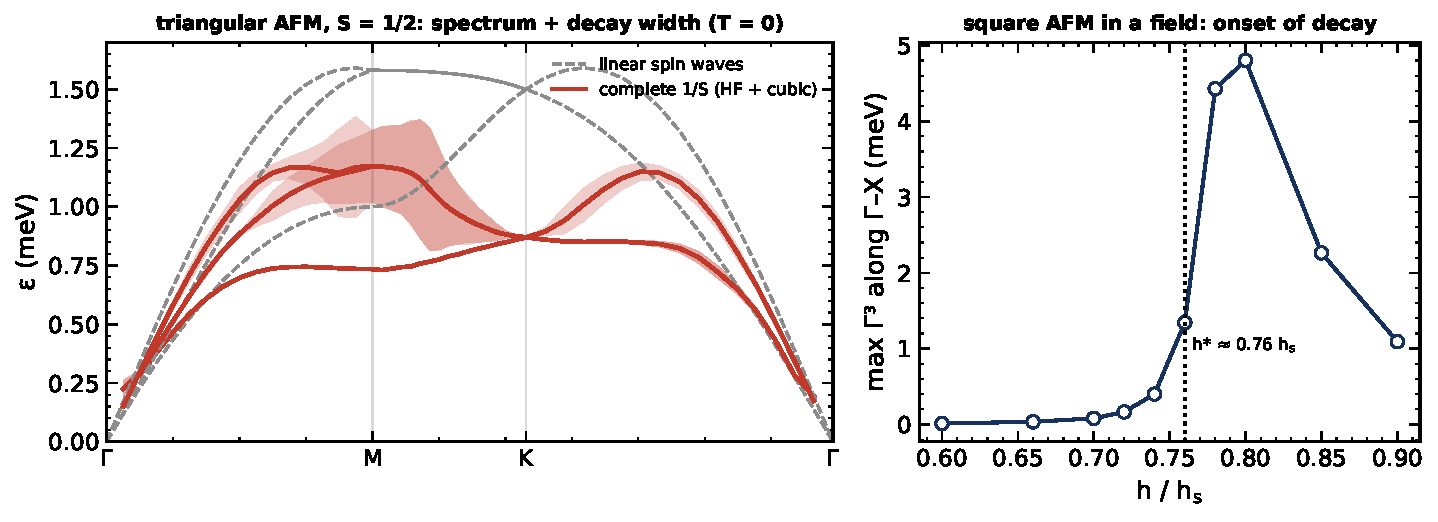
\includegraphics[width=0.86\textwidth]{figures/nonlinear.pdf}

{\tiny HP terms = exact classical expansion ($10^{-9}$); bubble+tadpole and sunset = exact diagonalisation of boson clusters ($10^{-6}$);
triangular: $c_\parallel(1-0.118/2S)$ vs $-0.115$ (Chubukov et al.), HF gap at $\pm K$ cancelled by $\Sigma^{(3)}$ (Goldstone); decay onset $h^*\approx0.76h_s$; FM: $\Gamma^{(4)}(T{=}0)=0$.}
\end{frame}

\begin{frame}{Self-consistent magnon decay}
\noindent{\footnotesize Born $\Gamma_k=-2\,\mathrm{Im}\,\Sigma^{(3)}(\varepsilon_k)$ is singular at decay thresholds. i$\Gamma$ approximation on a closed grid: resonant
channels $\omega-\varepsilon_q-\varepsilon_{k-q}+\tfrac{i}{2}(\textcolor{red!70!black}{\Gamma_q}+\textcolor{red!70!black}{\Gamma_{k-q}})$, $\textcolor{red!70!black}{\Gamma_k}=-2\,\mathrm{Im}\,\Sigma_k(E_k)$ iterated;
$E_k$ = the \textcolor{spinc}{$1/S$} on-shell energy (keeps the HF/cubic Goldstone cancellation). \cmd{--cubic --sc-decay}.}
\vspace{0.2em}

\centering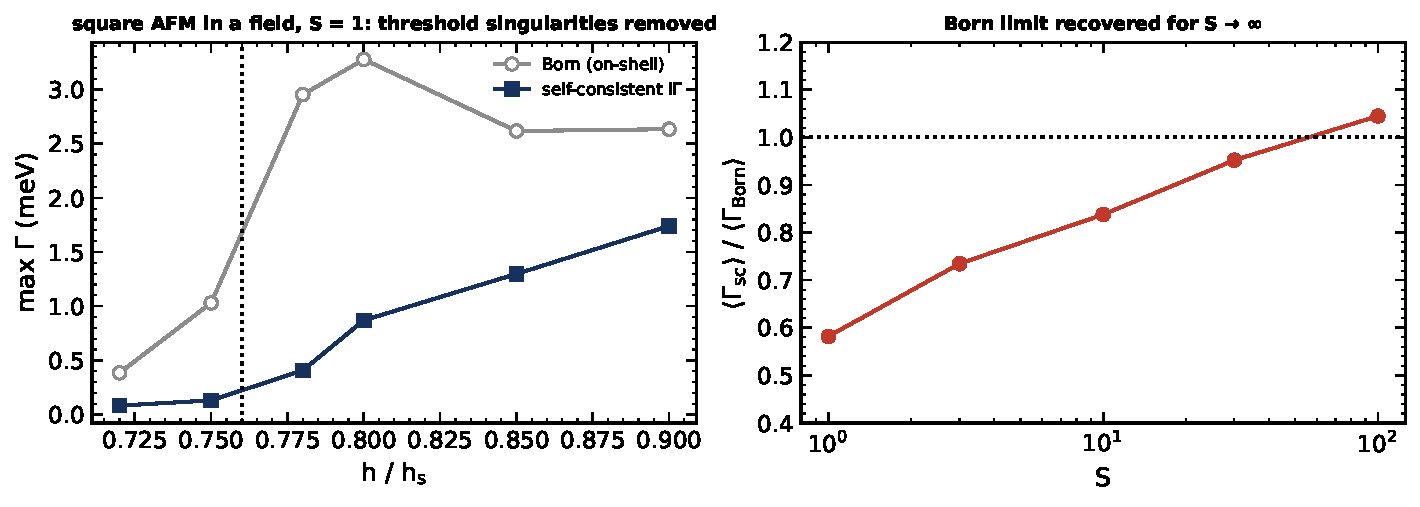
\includegraphics[width=0.86\textwidth]{figures/scdecay.pdf}

{\tiny On-shell mode $=$ Born to $10^{-10}$; fixed-point residual $\sim10^{-6}$ meV; $\langle\Gamma_{sc}\rangle/\langle\Gamma_{\rm Born}\rangle\to1$ for $S\to\infty$; triangular AFM: Goldstone branches stay
underdamped ($\Gamma/E<0.01$) with short-tailed widths (Lorentzian tails: $\Gamma/E\approx2$); off-shell Dyson breaks Goldstone.}
\end{frame}

\begin{frame}[fragile]{Spin–orbit-torque geometry: unconventional polarisations}
\begin{columns}[T]
\column{0.5\textwidth}
For every current flow $i$ $\perp$ field $j$ SymPhase lists the allowed spin (orbital) polarisations:
\begin{lstlisting}
allowed polarisations (flow i, field j):
  flow x, E || y : S_{z}
  flow x, E || z : S_{y}
  flow z, E || x : S_{y}
  flow z, E || y : S_{x}
\end{lstlisting}
\small Conventional SHE: $\Sv\perp$ flow $\perp$ field. Any additional entry
(e.g.\ $\Sv_z$ for flow $z$, $\Ef\parallel x$) is an \textbf{unconventional} torque channel — field-free switching.
\column{0.46\textwidth}
\begin{tcolorbox}[sp,title=Typical use (interfaces)]
\begin{itemize}\setlength\itemsep{0.25em}
  \item slab with heavy metal / magnet (Ni, NbP, CrSb, Mn$_3$Sn …)
  \item $\Top$-even block: intrinsic (Fermi-sea) torques
  \item $\Top$-odd block: magnetic / Fermi-surface ($\propto 1/\Gamma$)
  \item orbital tensor: same shape, different magnitude
\end{itemize}
\end{tcolorbox}
\end{columns}
\end{frame}

% =============================================================================
\sectionslide{5 \; Convex hull}{thermodynamic stability for any number of elements}

\begin{frame}{Thermodynamics on one slide}
\begin{columns}[T]
\column{0.52\textwidth}
\[
\Eform = \frac{\Etot - \sum_i n_i\,\muzero_i}{\sum_i n_i}
\]
\begin{itemize}\setlength\itemsep{0.4em}
  \item hull = lower convex envelope of $(\mathbf x,\Eform)$ in the composition simplex (Qhull)
  \item $\Ehull\ge0$: energy released on decomposing into hull phases (lever rule)
  \item \textbf{stability margin}: depth of a stable phase below the hull of all other phases
  \item hull energy at any composition, pseudo-binary cuts $\mathbf x(t)=(1-t)\mathbf x_A+t\,\mathbf x_B$
\end{itemize}
\column{0.45\textwidth}
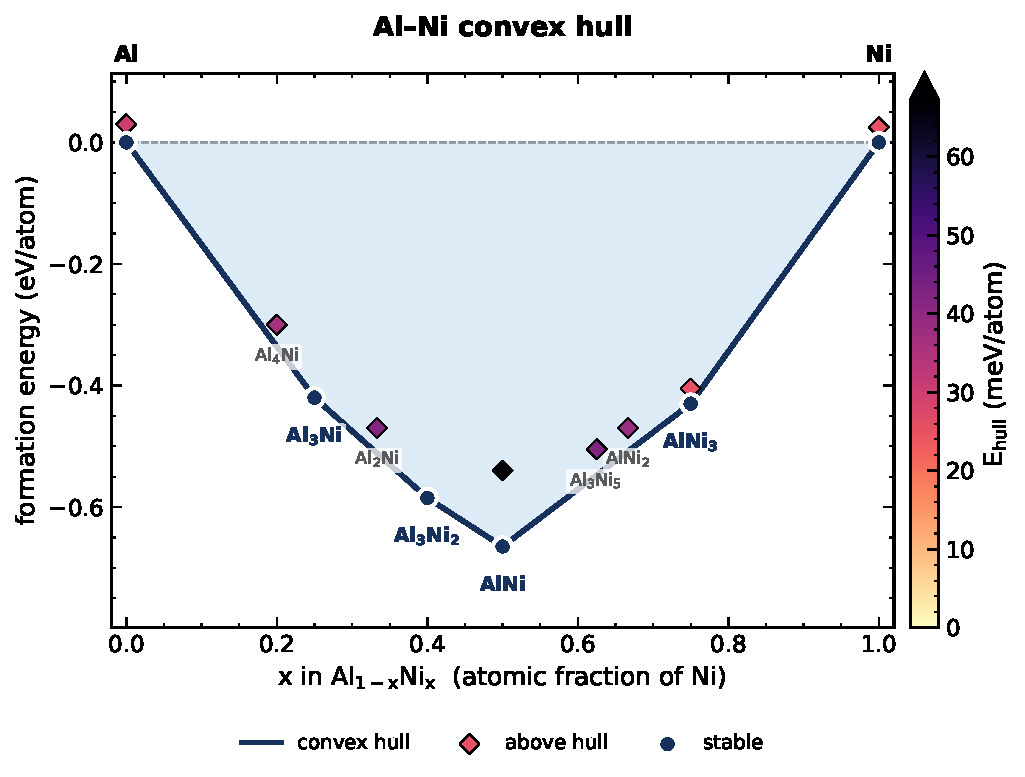
\includegraphics[width=\linewidth]{figures/binary.pdf}
\end{columns}
\end{frame}

\begin{frame}{Ternary: Gibbs triangle and 3D hull surface}
\begin{columns}[c]
\column{0.5\textwidth}
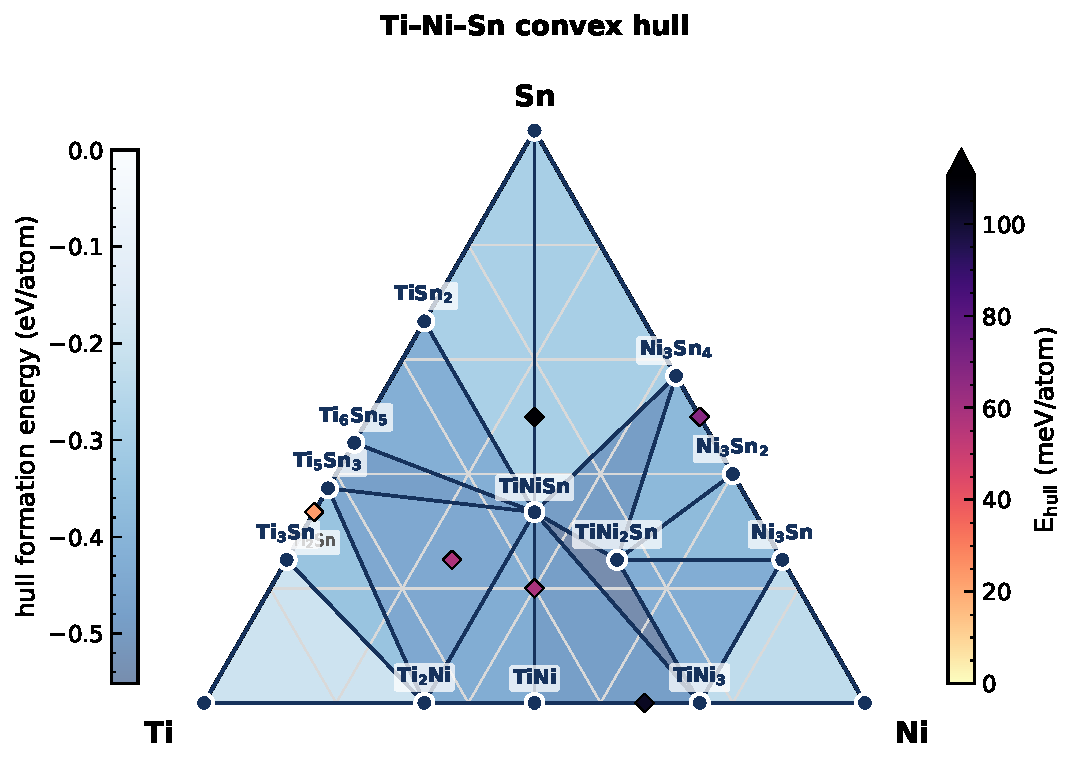
\includegraphics[width=\linewidth]{figures/ternary.pdf}
\column{0.5\textwidth}
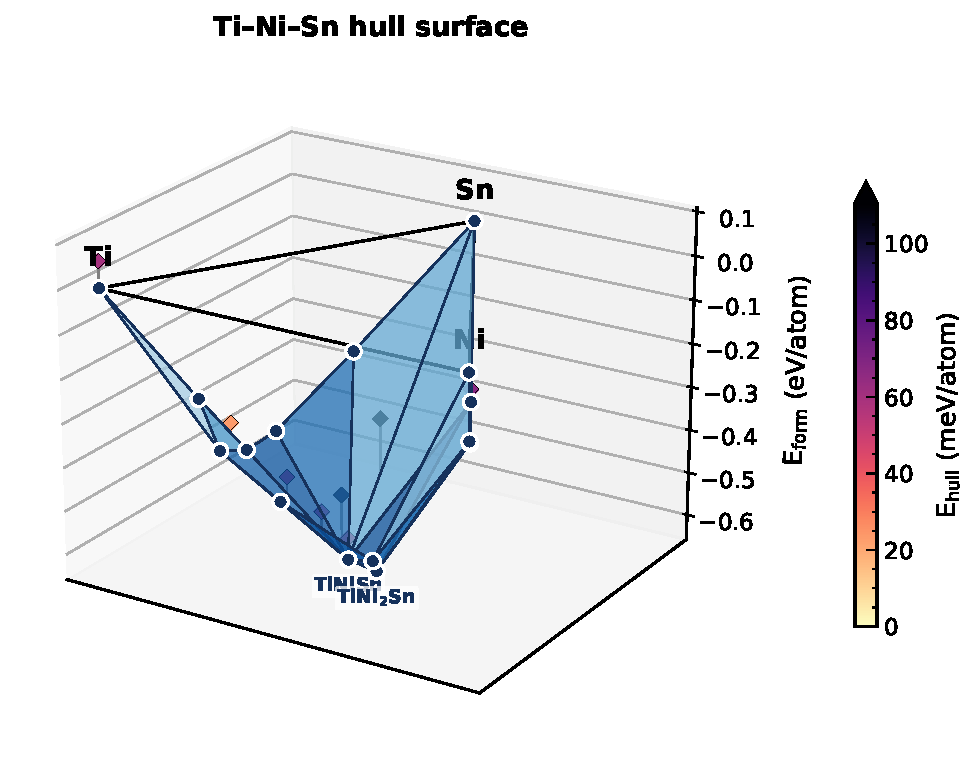
\includegraphics[width=\linewidth]{figures/surface.pdf}
\end{columns}
\vspace{-0.3em}
{\scriptsize\color{greyt} toy energies (teaching data set shipped with SymPhase). Shaded triangles: three-phase facets; lines: tie-lines; diamonds: $\Ehull$ colour scale.}
\end{frame}

\begin{frame}{Four and more elements}
\begin{columns}[c]
\column{0.40\textwidth}
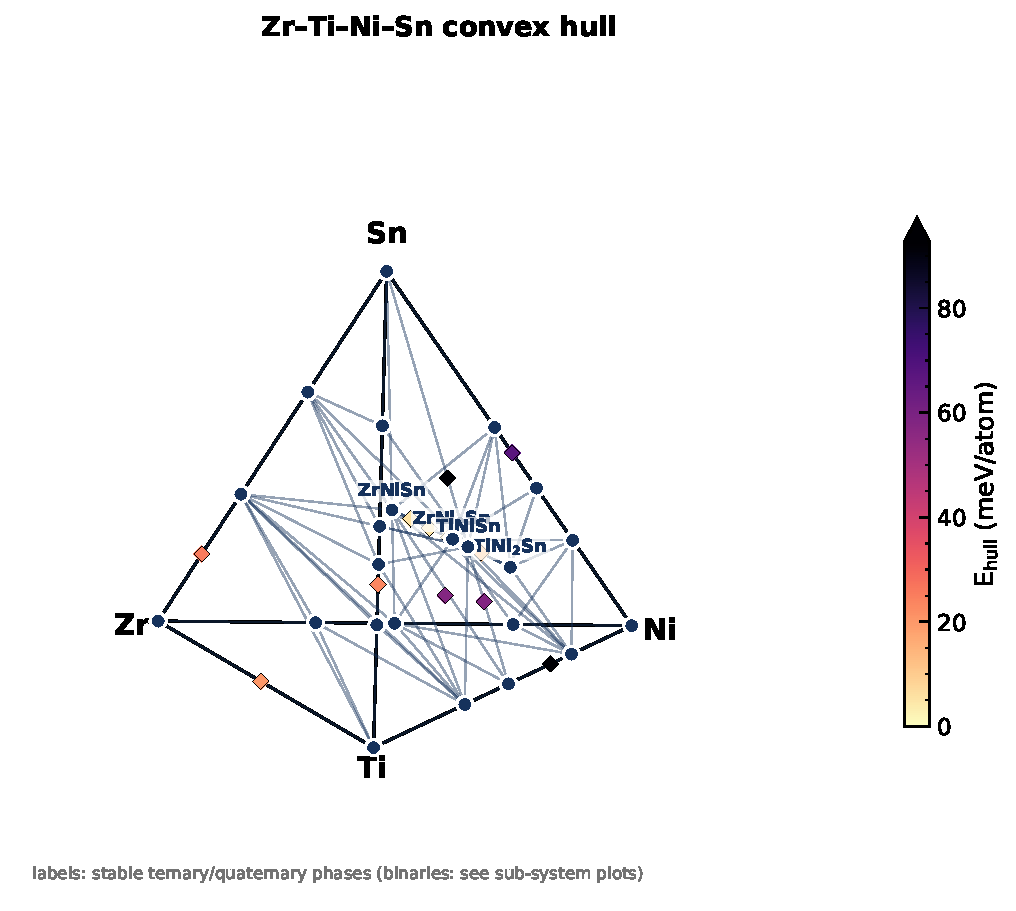
\includegraphics[width=\linewidth,height=0.72\textheight,keepaspectratio]{figures/quaternary.pdf}
\column{0.60\textwidth}
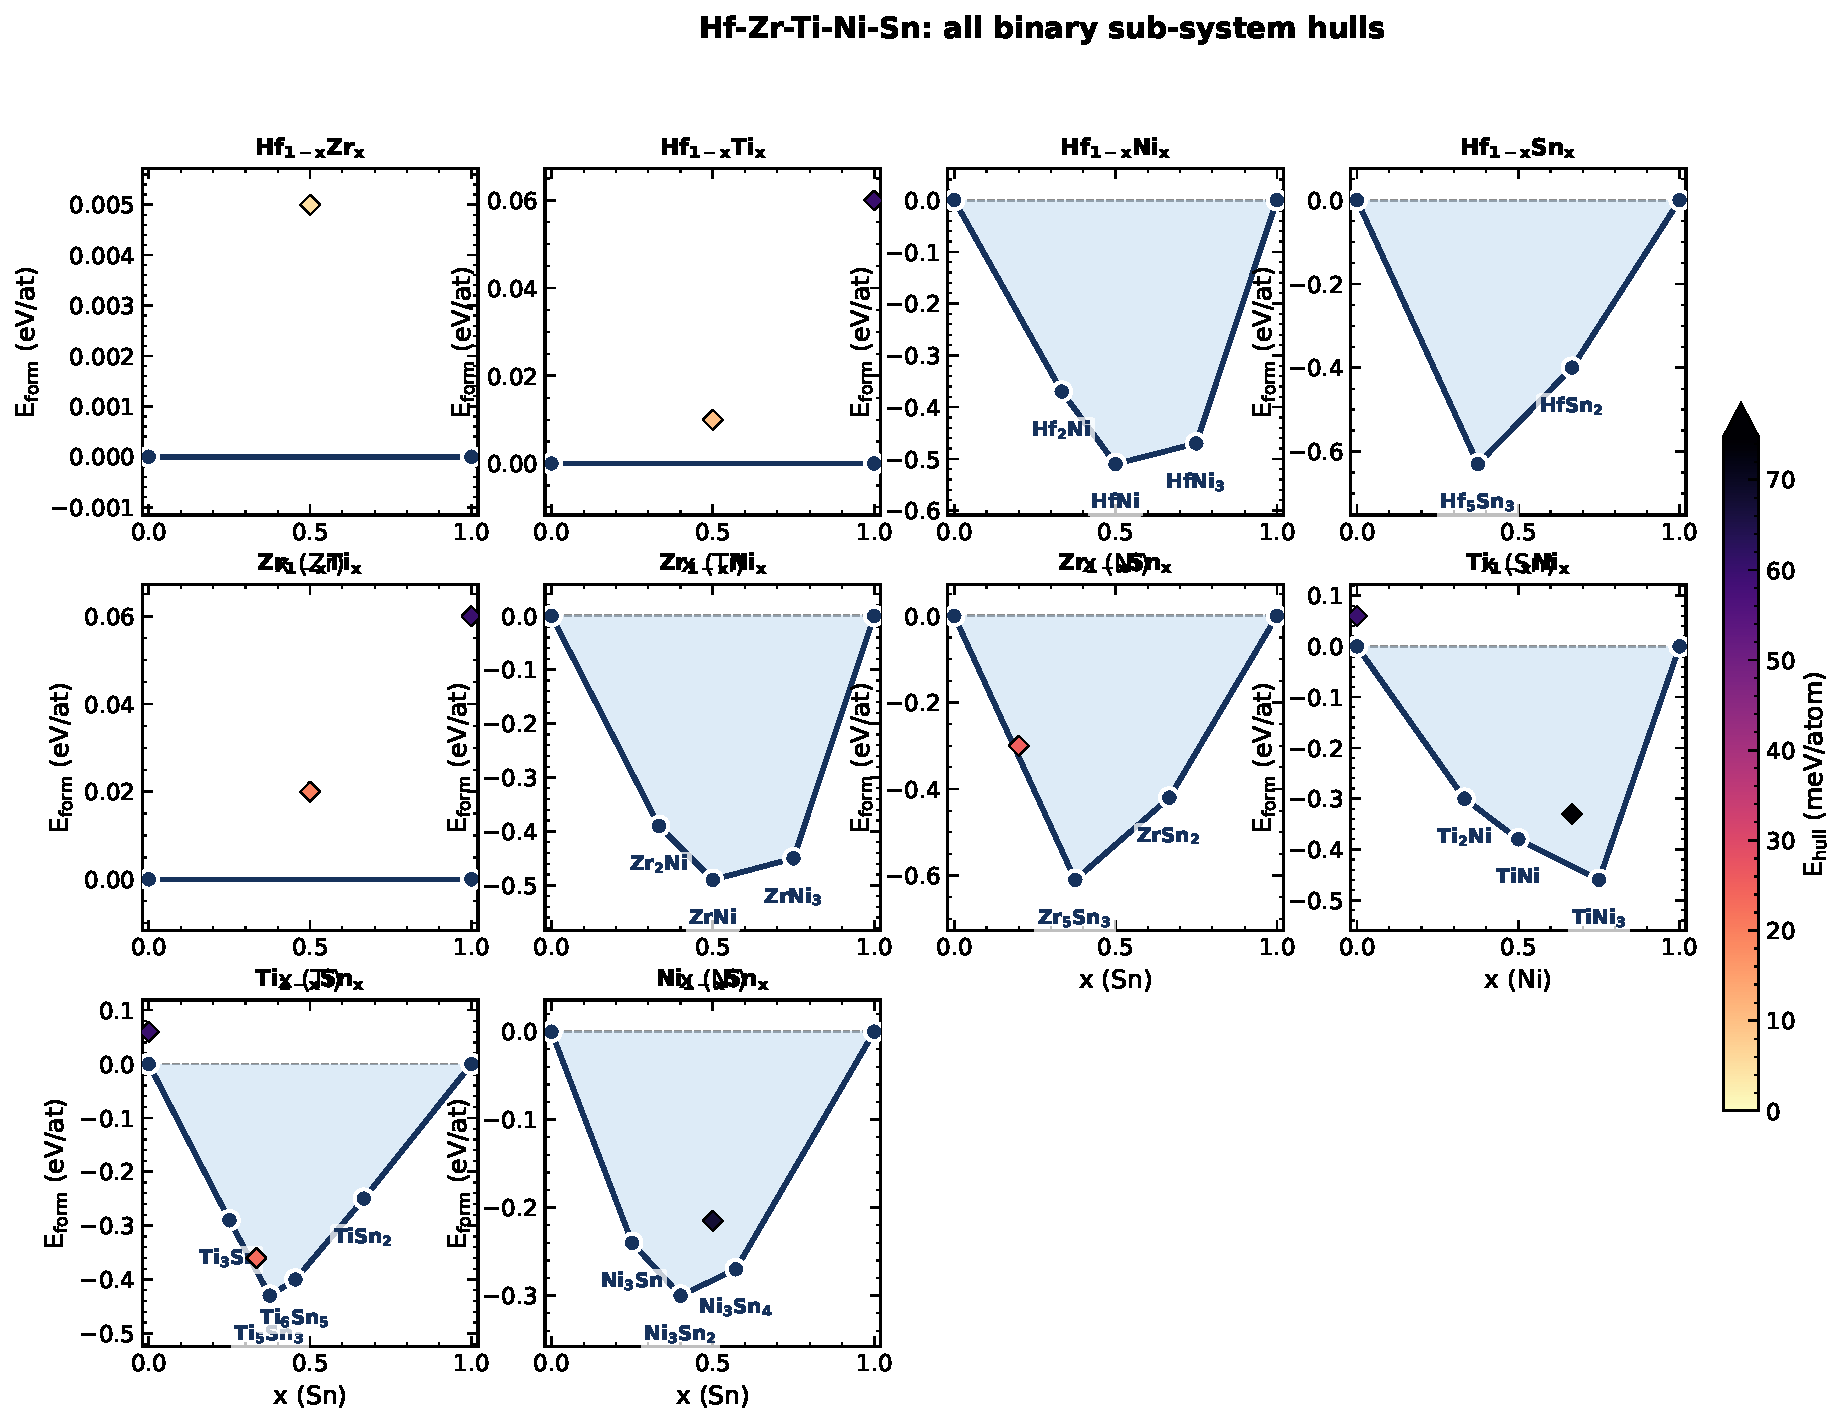
\includegraphics[width=\linewidth,height=0.74\textheight,keepaspectratio]{figures/sub5.pdf}
\end{columns}
\vspace{-0.3em}
{\small Quaternary: tetrahedron with tie-lines. $n\ge5$: grid of all binary (or ternary) sub-hulls, here Ti–Zr–Hf–Ni–Sn.}
\end{frame}

\begin{frame}{Pseudo-binary slices, $\Ehull$ ranking and screening}
\begin{columns}[c]
\column{0.52\textwidth}
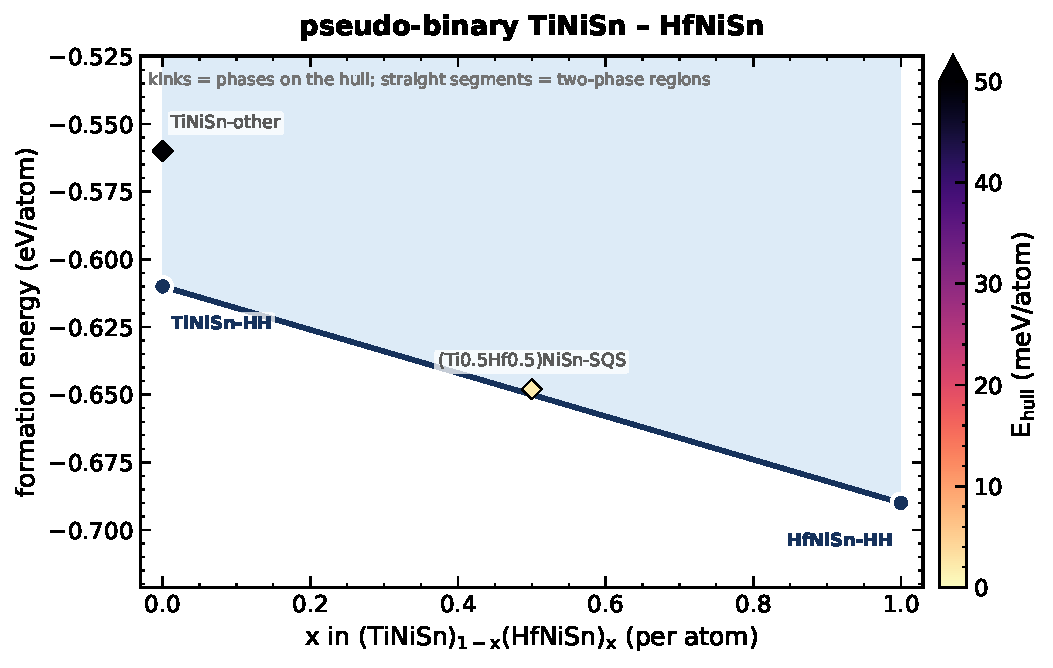
\includegraphics[width=\linewidth,height=0.6\textheight,keepaspectratio]{figures/slice.pdf}
\column{0.46\textwidth}\centering
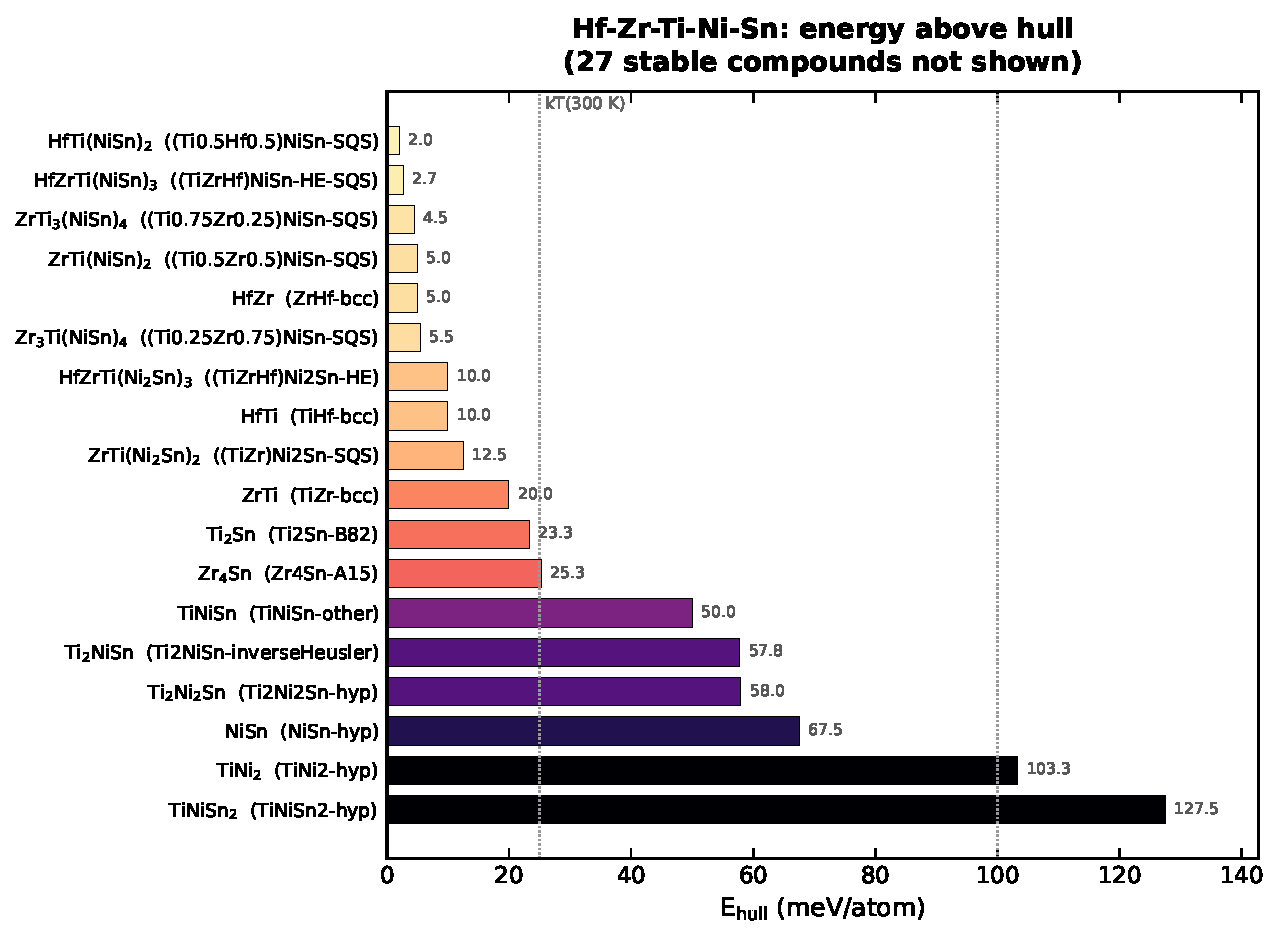
\includegraphics[width=\linewidth,height=0.64\textheight,keepaspectratio]{figures/ehull_bar.pdf}
\end{columns}
\begin{tcolorbox}[sp]
\texttt{h.evaluate\_many(candidates)} / \cmd{symphase hull --screen cand.csv}: $\Ehull$ and decomposition of
thousands of hypothetical compounds against a fixed hull, in parallel.
\end{tcolorbox}
\end{frame}

% =============================================================================
\begin{frame}{Finite-temperature hulls}
\begin{columns}[c]
\column{0.36\textwidth}
\[
\textcolor{enc}{G_i(T)}=\textcolor{enc}{E_i}+\textcolor{enc}{F^{\rm vib}_i(T)}-T\,S^{\rm conf}_i
\]
{\footnotesize
\begin{itemize}\setlength\itemsep{0.15em}
 \item $S^{\rm conf}$ from sublattices: \texttt{Ti0.5Zr0.5|Ni|Sn} $\to k_B\ln2/3$
 \item $F^{\rm vib}$: Debye, phonopy (DOS or \texttt{thermal\_properties.yaml}), Bartel SISSO
 \item hull rebuilt at every $T$; $T_{\rm stab}$ by bisection
\end{itemize}}
\begin{tcolorbox}[hl]
(Ti$_{0.5}$Zr$_{0.5}$)NiSn: $\Ehull=5$ meV/atom $\Rightarrow T^*=251$ K (analytic: 251.1 K)
\end{tcolorbox}
\column{0.62\textwidth}
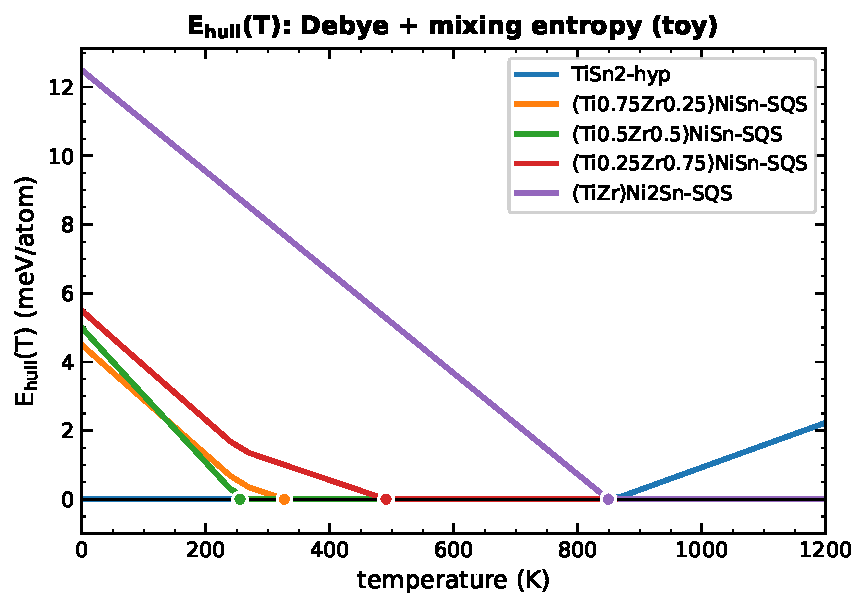
\includegraphics[width=\linewidth]{figures/ehull_vs_T.pdf}
\end{columns}
\end{frame}

\sectionslide{6 \; Elements in, everything out}{\texttt{symphase run Ti Ni Sn}}

\begin{frame}[fragile]{MXenes and 2D materials: \texttt{symphase mxene}}
\begin{columns}[T]
\column{0.44\textwidth}
\begin{lstlisting}[basicstyle=\ttfamily\tiny]
$ symphase mxene --hull
  transition metal M: Cr
  X element (C or N) [C]: C
  n in M(n+1)X(n) [1]: 1
  passivation (F,O,OH,Cl,none) [F]: F
  termination site [auto]: auto
  Cr2CF2 site fcc: E = -7.9139 eV/atom
  Cr2CF2 site hcp: E = -7.8091 eV/atom
  Cr2CF2: E_hull = 265 meV/atom
     -> Cr7C3 + C + CrF2
\end{lstlisting}
\column{0.54\textwidth}
{\tiny\renewcommand{\arraystretch}{1.1}\setlength{\tabcolsep}{3pt}
\begin{tabular}{@{}lccccc@{}}
\toprule
2D & $a$ (Å) & site & $\Eform$ (eV/at) & $\Ehull$ (meV/at) & $\Delta\mu_F^*$ (eV)\\
\midrule
Cr$_2$CF$_2$ & 2.955 & fcc & $-1.445$ & 265 & $-3.90$\\
Ni$_2$NF$_2$ & 3.029 & fcc & $-0.959$ & 377 & $-2.92$\\
Mo$_2$C      & 2.971 & —   & $+0.212$ & 391 & $-2.95$\\
\bottomrule
\end{tabular}

\vspace{0.4em}
\texttt{symphase.twod}: $M_{n+1}X_nT_2$ builder (asks for $M$, $X$, $n$, passivation; double-$M$; OH), fcc/hcp/top sites,
layer detection, monolayer from bulk, exfoliation energy, in-plane relaxation, VASP inputs, hull, phase diagrams.
Energies: CHGNet (MP PBE/PBE+U scale); hcp termination +105/+101 meV/atom.\par}
\end{columns}

\vspace{0.1em}
\centering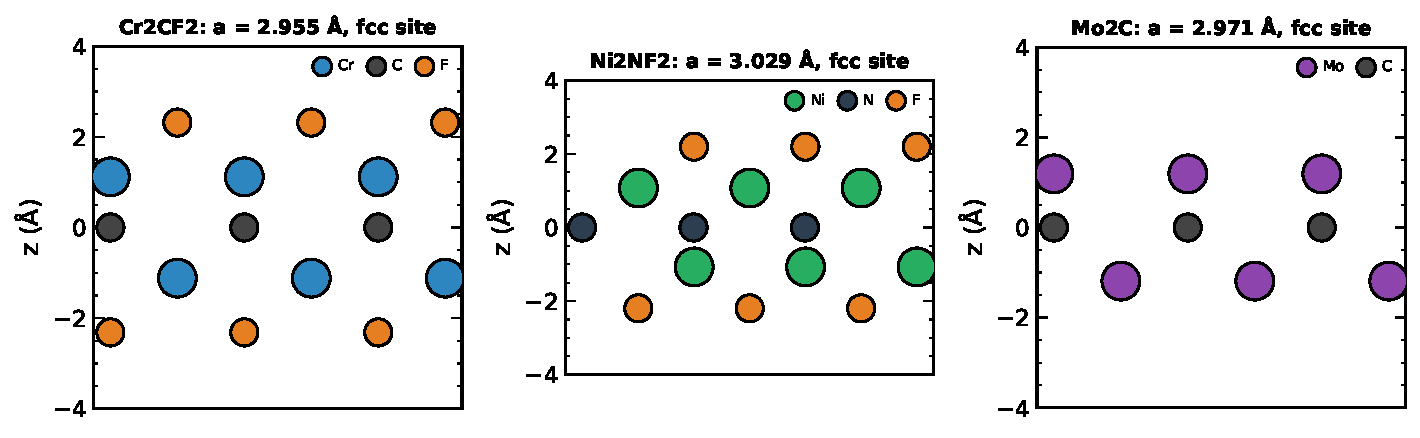
\includegraphics[width=0.8\textwidth]{figures/mxene_structures.pdf}
\end{frame}

\begin{frame}{MXene convex hulls and termination phase diagram}
\centering
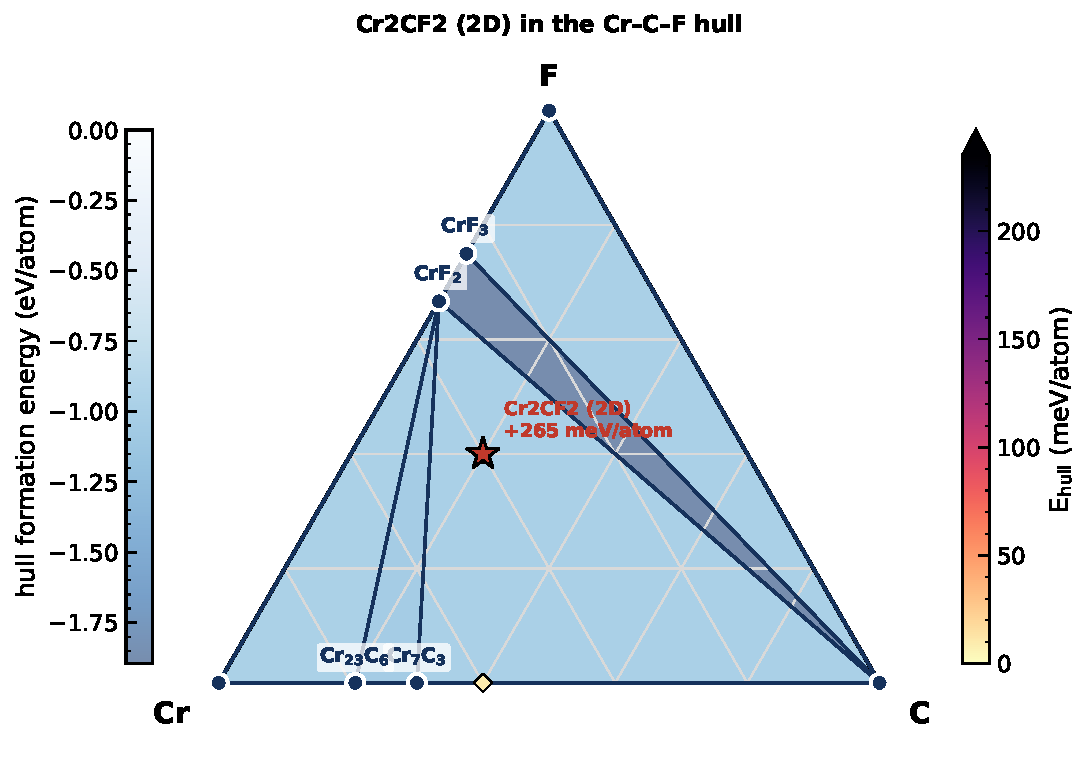
\includegraphics[width=0.325\textwidth]{figures/mxene_pd_Cr2CF2.pdf}\hfill
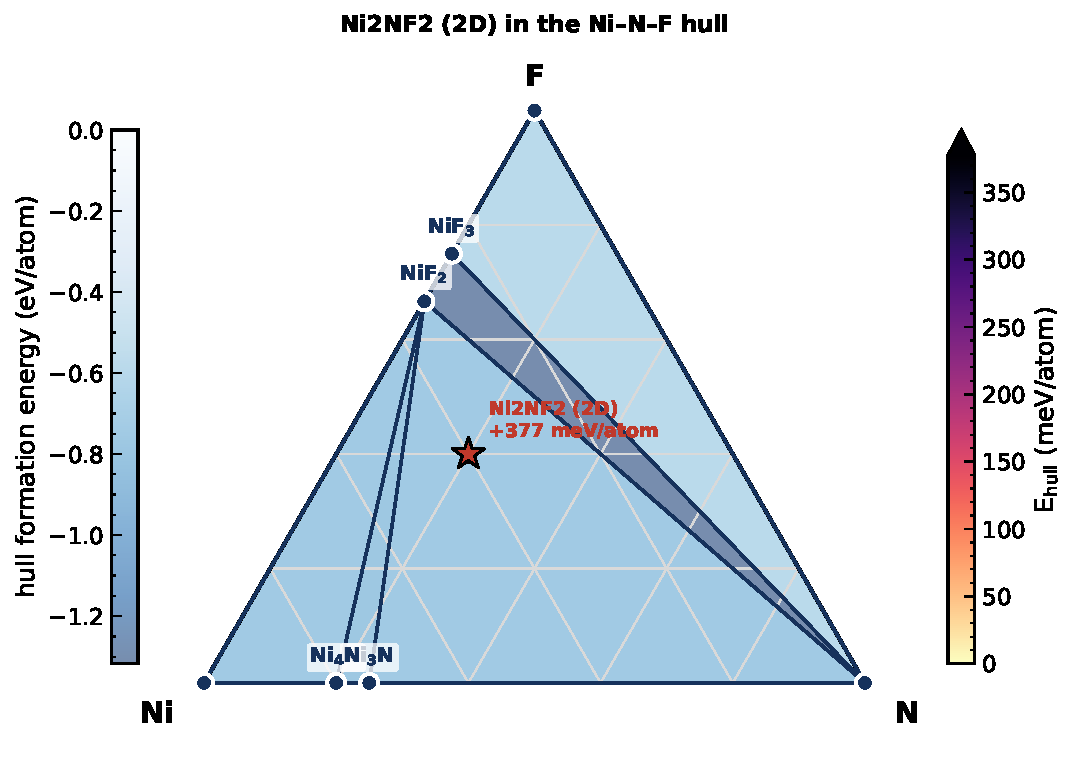
\includegraphics[width=0.325\textwidth]{figures/mxene_pd_Ni2NF2.pdf}\hfill
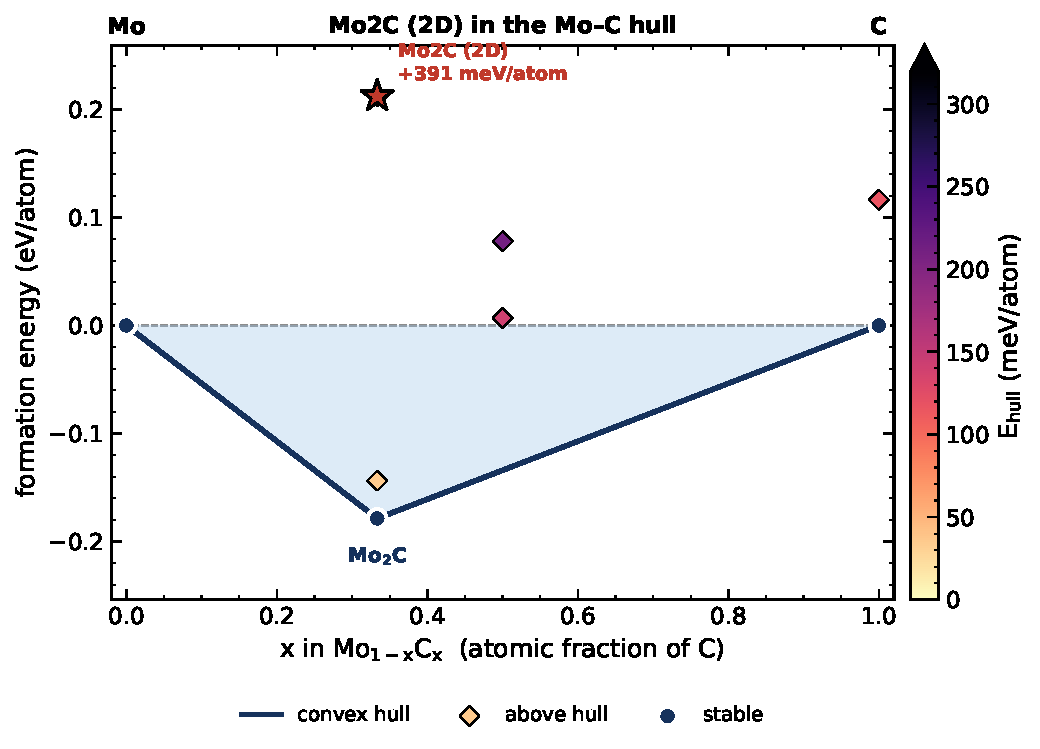
\includegraphics[width=0.325\textwidth]{figures/mxene_pd_Mo2C.pdf}

\vspace{0.1em}
\begin{columns}[T]
\column{0.36\textwidth}
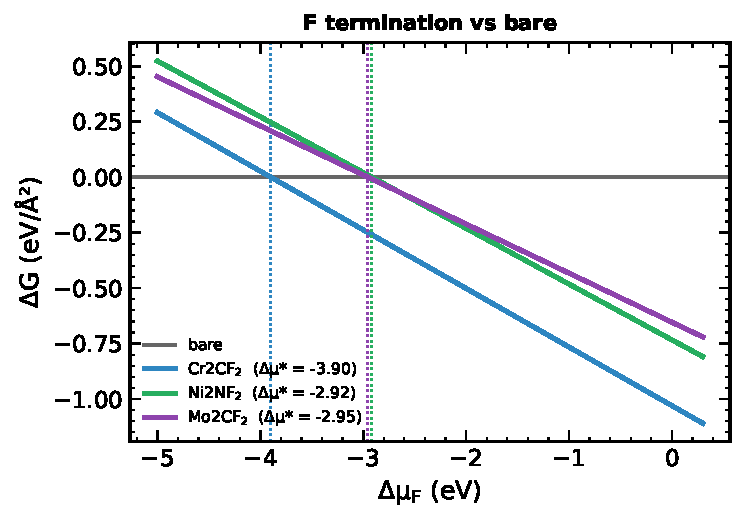
\includegraphics[width=\linewidth]{figures/mxene_termination.pdf}
\column{0.62\textwidth}
{\tiny
\begin{itemize}\setlength\itemsep{0.05em}
\item metastable monolayers, $\Ehull$ = 265–391 meV/atom: Cr$_2$CF$_2\to$ Cr$_7$C$_3$ + C + CrF$_2$; Ni$_2$NF$_2\to$ Ni$_3$N + N$_2$ + NiF$_2$;
Mo$_2$C(2D)$\to$ bulk $\beta$-Mo$_2$C
\item F termination wins for $\Delta\mu_F > \Delta\mu_F^*$ = $-3.9$, $-2.9$, $-3.0$ eV: fluorinated under etching conditions
\item bulk $\Eform$ (exp.): CrF$_2$ $-2.75$ ($-2.69$), CrF$_3$ $-2.93$ ($-3.00$), NiF$_2$ $-2.21$ ($-2.25$), Cr$_3$C$_2$ $-0.16$ ($-0.18$),
Cr$_7$C$_3$ $-0.20$ ($-0.17$), Mo$_2$C $-0.18$ ($-0.16$) eV/atom; MoC underbound, Ni$_3$N overbound
\item screening quality: confirm with VASP (\texttt{--vasp} inputs, \texttt{--energies} CSV)
\end{itemize}}
\end{columns}
\end{frame}

\begin{frame}[fragile]{The automatic pipeline}
\begin{columns}[T]
\column{0.42\textwidth}
\textbf{Input file} (\texttt{symphase.in}):
\begin{lstlisting}
elements = Ti Ni Sn
\end{lstlisting}
optional: \texttt{ehull\_window}, \texttt{write\_vasp}, \texttt{source}, Ibex settings …\\[0.5em]
\textbf{Output folder}
\begin{lstlisting}
symphase_Ni-Sn-Ti/
  SUMMARY.html  SUMMARY.md
  hull_table.csv  hull.json
  figures/   structures/
  vasp/  (INCAR KPOINTS POSCAR
          POTCAR.spec, submit_ibex.sh)
  data/  (cached database entries)
\end{lstlisting}
\column{0.55\textwidth}
\centering
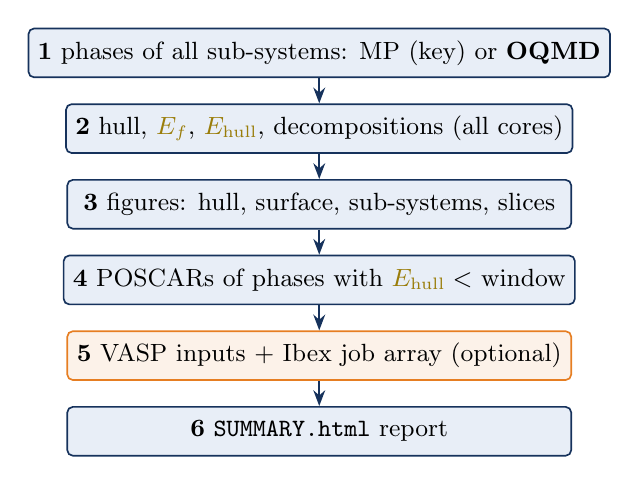
\begin{tikzpicture}[font=\small,node distance=0.32cm,
  st/.style={draw=navy,fill=navylight,rounded corners=2pt,minimum width=6.4cm,minimum height=0.62cm,align=left,line width=0.6pt},
  arr/.style={-{Stealth[length=2mm]},navy,line width=0.8pt}]
  \node[st] (a) {\textbf{1} phases of all sub-systems: MP (key) or \textbf{OQMD}};
  \node[st,below=of a] (b) {\textbf{2} hull, $\Eform$, $\Ehull$, decompositions (all cores)};
  \node[st,below=of b] (c) {\textbf{3} figures: hull, surface, sub-systems, slices};
  \node[st,below=of c] (d) {\textbf{4} POSCARs of phases with $\Ehull<$ window};
  \node[st,below=of d,fill=accent!10,draw=accent] (e) {\textbf{5} VASP inputs + Ibex job array (optional)};
  \node[st,below=of e] (f) {\textbf{6} \texttt{SUMMARY.html} report};
  \foreach \x/\y in {a/b,b/c,c/d,d/e,e/f} \draw[arr] (\x)--(\y);
\end{tikzpicture}
\end{columns}
\end{frame}

\begin{frame}[fragile]{From database phases to your own DFT on Ibex}
\begin{columns}[T]
\column{0.5\textwidth}
\begin{lstlisting}[language=bash]
# login node (internet), ~1 min
symphase run Ti Ni Sn write_vasp=yes
cd symphase_Ni-Sn-Ti/vasp
./submit_ibex.sh      # POTCARs + job array
# ... jobs finished:
symphase run Ti Ni Sn source=vasp \
     vasp_dir=symphase_Ni-Sn-Ti/vasp
# tensors of any finished run
cd 01_TiNiSn_*/ && symphase tensors
\end{lstlisting}
\column{0.46\textwidth}
\textbf{Generated job script}
\begin{itemize}\setlength\itemsep{0.25em}
  \item \texttt{--array=0-N\%10}, \texttt{largemem}, 40 tasks
  \item oneAPI \texttt{setvars.sh} (guarded by \texttt{set +e})
  \item POTCARs built on the login node from \texttt{potpaw\_PBE} (MP-recommended PAWs)
  \item MAGMOM, POSCAR and POTCAR orders consistent
  \item restart-safe: finished runs skipped
\end{itemize}
\begin{tcolorbox}[hl]
second pass: hull purely from \textbf{your} energies (same settings for every phase).
\end{tcolorbox}
\end{columns}
\end{frame}

% =============================================================================
\sectionslide{7 \; Parallel engine}{any number of cores, any number of nodes}

\begin{frame}[fragile]{What runs in parallel}
\begin{columns}[T]
\column{0.5\textwidth}
\renewcommand{\arraystretch}{1.2}\small\setlength{\tabcolsep}{4pt}
\begin{tabular}{@{}ll@{}}
\toprule
task & parallel over \\ \midrule
$\Ehull$, decomposition, margin & entries \\
screening (\texttt{--screen}) & candidates \\
VASP folder parsing (\texttt{--scan}) & run directories \\
pseudo-binary hull & composition points \\
symmetry of near-hull phases & structures \\
Qhull construction & serial (fast) \\ \bottomrule
\end{tabular}
\vspace{0.5em}

{\small\textbf{Backends}: \texttt{process} (fork, copy-on-write, no pickling of the hull), \texttt{mpi} (mpi4py, round-robin + allgather), \texttt{serial}. Results identical to serial (tested).}
\column{0.46\textwidth}
\begin{lstlisting}[language=bash]
# one node, all 40 cores
symphase hull --scan calcs/ -n 40
sbatch jobs/ibex_symphase.slurm

# 4 nodes x 40 ranks
srun -n 160 python -m symphase hull \
     --csv refs.csv --screen big.csv
sbatch jobs/ibex_symphase_mpi.slurm
\end{lstlisting}
\small Cores: \texttt{-n}, \texttt{SYMPHASE\_NPROC}, \texttt{SLURM\_CPUS\_PER\_TASK}, CPU affinity. BLAS threads pinned to 1 per worker.
\end{columns}
\end{frame}

% =============================================================================
\sectionslide{8 \; Learning material}{tutorials, quizzes, validation}

\begin{frame}{Tutorial and quiz notebooks}
\begin{columns}[T]
\column{0.58\textwidth}
\renewcommand{\arraystretch}{1.25}
{\scriptsize\renewcommand{\arraystretch}{0.74}\begin{tabular}{@{}l>{\raggedright\arraybackslash}p{6.0cm}@{}}
\toprule
notebook & content\\ \midrule
01 & symmetry \& tensors: Pt, Fe, RuO$_2$, MoO$_2$, spin groups \\
02 & hull: 2--5 elements, slices, screening, benchmark\\
03 & elements-only pipeline, Ibex workflow\\
06 & SSG numbers, magnon chirality (RuO$_2$)\\
07 & finite-$T$ hulls: mixing entropy, phonons\\
08 & non-collinear FM/AFM: triangular, canted DMI\\
10 & incommensurate spirals (rotating frame)\\
12 & supercells: multi-Q, conical, distorted\\
14 & OSSG numbers, magnon–phonon coupling\\
15 & quasi-harmonic \& anharmonic hulls\\
17 & Kubo magnitudes with symmetry\\
18 & TDEP / SSCHA anharmonic phonons\\
20 & two-magnon striction, damping\\
22 & four-magnon HF, self-energies\\
24 & cubic terms, four-magnon damping\\
26 & self-consistent magnon decay\\
28 & MXenes / 2D: hulls, phase diagrams\\
quizzes & \textbf{12 $\times$ 20 q.}: 04, 05, 09, 11, 13, 16, 19, 21, 23, 25, 27, 29\\ \bottomrule
\end{tabular}}
\column{0.4\textwidth}
\begin{tcolorbox}[sp,title=Self-checking quizzes]
\texttt{q = Quiz("hull")}\\
\texttt{q.answer(10, 42.5)} $\to$ \textcolor{spinc}{\checkmark} + explanation\\
\texttt{q.hint(n)}, \texttt{q.reveal(n)}, \texttt{q.score()}\\
\texttt{q.widget(n)} clickable (ipywidgets)
\end{tcolorbox}
Conceptual + hands-on questions; hands-on answers are computed by SymPhase on the shipped examples.
\end{columns}
\end{frame}

\begin{frame}{Validation}
\renewcommand{\arraystretch}{0.8}
\centering\tiny
\begin{tabular}{@{}p{4.6cm}p{6.9cm}c@{}}
\toprule
test & expected & ok \\ \midrule
fcc Pt & $Fm\bar3m1'$, 1 SHE component, no AHE & \textcolor{spinc}{\checkmark} \\
bcc Fe, $\mathbf m\parallel z$ & $I4/mm'm'$, $\mathbf h\parallel z$ & \textcolor{spinc}{\checkmark} \\
RuO$_2$, Néel $\parallel[001]$ & $P4_2'/mnm'$, no AHE, spin splitter & \textcolor{spinc}{\checkmark} \\
RuO$_2$, Néel $\parallel[100]$ & $Pnn'm'$, AHE allowed & \textcolor{spinc}{\checkmark} \\
non-collinear, \texttt{SAXIS}$\parallel x$ & moments rotated to $x$ & \textcolor{spinc}{\checkmark} \\
hull: process / MPI & identical to serial & \textcolor{spinc}{\checkmark} \\
Ibex script & file orders consistent, array dry run & \textcolor{spinc}{\checkmark} \\
spin groups (RuO$_2$, MnTe, Cr, Mn$_2$Au) & d-wave, g-wave, AFM, PT-AFM & \textcolor{spinc}{\checkmark} \\
INCAR \texttt{SAXIS} rotation & Néel $\to x$: $Pnn'm'$ & \textcolor{spinc}{\checkmark} \\
MoO$_2$ ($P2_1/c$) & $2/m1'$, 13 SHE/OHE comps (odd-$y$ rule) & \textcolor{spinc}{\checkmark} \\
SSG numbers (5 examples) & BNS of C$_{2\perp}\!\to\!\Top$ group, \texttt{spinspg} & \textcolor{spinc}{\checkmark} \\
magnons: FM, AFM chain, RuO$_2$ & analytic $\omega(\mathbf q)$; d-wave $\Delta\omega$ & \textcolor{spinc}{\checkmark} \\
finite-$T$ hull & $T^*=251$ K (analytic), Debye limits & \textcolor{spinc}{\checkmark} \\
non-collinear LSWT & FM[111], 120° triangular, canted DMI & \textcolor{spinc}{\checkmark} \\
incommensurate spirals & J$_1$–J$_2$, DMI helix, 6-site supercell & \textcolor{spinc}{\checkmark} \\
supercells & cone angle (analytic), SkX $N_{sk}=-3$, exact mapping & \textcolor{spinc}{\checkmark} \\
OSSG numbers (6 orders) & MSG of FindSpinGroup = SymPhase & \textcolor{spinc}{\checkmark} \\
magnon–phonon & two-oscillator formula, phonopy $\Phi$ = springs & \textcolor{spinc}{\checkmark} \\
QHA & \texttt{PhonopyQHA}; $\gamma=0$, Grüneisen relation & \textcolor{spinc}{\checkmark} \\
Kubo & Haldane, Kane–Mele quantised; 3D units & \textcolor{spinc}{\checkmark} \\
TDEP / SSCHA & exact oscillator, Gibbs–Bogoliubov bound & \textcolor{spinc}{\checkmark} \\
two-magnon / damping & frozen-phonon supercell, 1D roots, FM/AFM LLG & \textcolor{spinc}{\checkmark} \\
four-magnon HF & Dyson FM, Oguchi chain/square, 1D breakdown & \textcolor{spinc}{\checkmark} \\
self-energies & $-2\,\mathrm{Im}\,\Sigma=\gamma$ golden rule, $\int A=1$ & \textcolor{spinc}{\checkmark} \\
cubic + sunset & = classical expansion, = exact diagonalisation, $c_\parallel$ & \textcolor{spinc}{\checkmark} \\
self-consistent decay & Born limit (on-shell, $S\to\infty$), residual $10^{-6}$ & \textcolor{spinc}{\checkmark} \\
MXenes / 2D & HP builder, hulls reproducible, bulk $\Eform$ vs exp.\ ($\le$0.08 eV) & \textcolor{spinc}{\checkmark} \\
quiz keys & 240 / 240 self-consistent & \textcolor{spinc}{\checkmark} \\ \bottomrule
\end{tabular}
\vspace{0.2em}

{\scriptsize Automated tests: \texttt{pytest tests/} (97); OQMD/MP download checked with a mock server.}
\end{frame}

\begin{frame}{Limitations and outlook}
\begin{columns}[T]
\column{0.5\textwidth}
\textbf{Limitations}
\begin{itemize}\setlength\itemsep{0.35em}
  \item non-collinear OSSG numbers need the optional FindSpinGroup package (Python $\ge$ 3.11)
  \item symmetry gives the \emph{shape}, not the magnitude, of tensors
  \item LSWT harmonic; incommensurate multi-Q only as commensurate supercell approximants; exchange constants supplied by the user
  \item mixing energy sources requires identical DFT settings
\end{itemize}
\column{0.46\textwidth}
\textbf{Outlook}
\begin{itemize}\setlength\itemsep{0.35em}
  \item single-ion anisotropy at $O(1/S)$; self-consistent energies beyond $1/S$ (Goldstone-preserving)
  \item Edelstein, nonlinear Hall, torkance tensors
  \item Fermi-surface (1/$\Gamma$) Kubo terms and orbital Hall from \texttt{hr.dat} + $L$ matrices
  \item direct TDEP force-constant input (phonon dispersions at $T$)
\end{itemize}
\end{columns}
\end{frame}

\begin{frame}{References}
\scriptsize
\begin{itemize}\setlength\itemsep{0.25em}
  \item A. Togo, K. Shinohara, I. Tanaka, \emph{Spglib: a software library for crystal symmetry search}, Sci. Technol. Adv. Mater. Meth. \textbf{4}, 2384822 (2024).
  \item S. P. Ong \emph{et al.}, \emph{Python Materials Genomics (pymatgen)}, Comput. Mater. Sci. \textbf{68}, 314 (2013).
  \item H. T. Stokes, B. J. Campbell, ISO-MAG tables of magnetic space groups (BNS/OG labels).
  \item M. Seemann, D. Ködderitzsch, S. Wimmer, H. Ebert, \emph{Symmetry-imposed shape of linear response tensors}, Phys. Rev. B \textbf{92}, 155138 (2015).
  \item J. Železný \emph{et al.}, \emph{Spin-orbit torques in locally and globally noncentrosymmetric crystals}, Phys. Rev. B \textbf{95}, 014403 (2017).
  \item L. Šmejkal \emph{et al.}, \emph{Crystal time-reversal symmetry breaking and spontaneous Hall effect}, Sci. Adv. \textbf{6}, eaaz8809 (2020).
  \item L. Šmejkal, J. Sinova, T. Jungwirth, \emph{Emerging research landscape of altermagnetism}, Phys. Rev. X \textbf{12}, 040501 (2022).
  \item R. González-Hernández \emph{et al.}, \emph{Efficient electrical spin splitter based on nonrelativistic collinear antiferromagnetism}, Phys. Rev. Lett. \textbf{126}, 127701 (2021).
  \item J. E. Saal \emph{et al.}, JOM \textbf{65}, 1501 (2013); S. Kirklin \emph{et al.}, npj Comput. Mater. \textbf{1}, 15010 (2015) — OQMD.
  \item A. Jain \emph{et al.}, \emph{The Materials Project}, APL Mater. \textbf{1}, 011002 (2013).
\end{itemize}
\end{frame}

\begin{frame}[plain]
  \begin{tikzpicture}[remember picture,overlay]
    \fill[navy] (current page.south west) rectangle (current page.north east);
    \node[text=white,font=\fontsize{34}{38}\selectfont\bfseries] at ([yshift=1.2cm]current page.center) {Thank you};
    \node[text=white!85,font=\large\ttfamily] at ([yshift=-0.2cm]current page.center) {pip install -e .  \&\&  symphase run Ti Ni Sn};
    \node[text=white!70,font=\normalsize\ttfamily] at ([yshift=-1.2cm]current page.center) {github.com/Gokaran-Shukla/symphase};
    \fill[accent] ([yshift=-2.0cm,xshift=-3cm]current page.center) rectangle ++(6,0.06);
  \end{tikzpicture}
\end{frame}

\end{document}
